%%%%%%%%%%%%%%%%%%%%%%%%%%%%%%%%%%%%%%%%%%%%%%%%%%%%%%%%%%%%%%%%%%%%%%%%%%%%%%%%
%2345678901234567890123456789012345678901234567890123456789012345678901234567890
%        1         2         3         4         5         6         7         8

\documentclass[letterpaper, 10 pt, conference]{ieeeconf}  % Comment this line out if you need a4paper

%\documentclass[a4paper, 10pt, conference]{ieeeconf}      % Use this line for a4 paper

\IEEEoverridecommandlockouts                              % This command is only needed if 
                                                          % you want to use the \thanks command
\newcommand{\red}[1]{{\color{red} #1}}
\overrideIEEEmargins                                      % Needed to meet printer requirements.

%In case you encounter the following error:
%Error 1010 The PDF file may be corrupt (unable to open PDF file) OR
%Error 1000 An error occurred while parsing a contents stream. Unable to analyze the PDF file.
%This is a known problem with pdfLaTeX conversion filter. The file cannot be opened with acrobat reader
%Please use one of the alternatives below to circumvent this error by uncommenting one or the other
%\pdfobjcompresslevel=0
%\pdfminorversion=4

% See the \addtolength command later in the file to balance the column lengths
% on the last page of the document

% The following packages can be found on http:\\www.ctan.org
\usepackage{graphics} % for pdf, bitmapped graphics files
\usepackage{graphicx}
\usepackage{epsfig} % for postscript graphics files
\usepackage{caption}
\usepackage{soul}
\usepackage[makeroom]{cancel}% for strikethrough
%\usepackage{mathptmx} % assumes new font selection scheme installed
\usepackage{subcaption}% subfigures 
% \usepackage[font=small]{caption}
\usepackage{times} % assumes new font selection scheme installed
\usepackage{amsmath} % assumes amsmath package installed
\usepackage{amssymb}  % assumes amsmath package installed
\usepackage{bbm}
\usepackage[nocomma]{optidef}
\usepackage{tabularx}
\usepackage{multirow}
\usepackage{tablefootnote}
\usepackage{bm}
\providecommand{\bm}{\pmb}

\usepackage{cite}
%\usepackage[caption=false]{subfig}
\usepackage{subcaption}
\usepackage{hyperref}
\usepackage{cleveref}
\usepackage{booktabs}
% \usepackage{ntheorem}
\usepackage{amsthm}
\usepackage{sidecap}
\sidecaptionvpos{figure}{c}
\usepackage[font=small]{caption}
\captionsetup[figure]{name=Fig.} 
%\theoremstyle{break}
% \theoremstyle{plain}
% \theorembodyfont{\upshape}
\newtheorem{example}{Example}
\newtheorem{theorem}{Theorem}
% \newtheorem{proof}{Proof}[theorem]
\newtheorem{corollary}{Corollary}[theorem]
% \numberwithin{example}{section}
\usepackage[dvipsnames]{xcolor}

\usepackage[ruled,vlined]{algorithm2e}

\newcommand\xqed[1]{%
  \leavevmode\unskip\penalty9999 \hbox{}\nobreak\hfill
  \quad\hbox{#1}}
\newcommand\demo{\xqed{$\square$}}

\usepackage{xcolor}
\newcommand\todo[1]{\textbf{\textcolor{red}{TODO: #1}}}

\DeclareMathAlphabet{\mathcal}{OMS}{cmsy}{m}{n}
\setlength{\textfloatsep}{3pt plus 0pt minus 3pt}
\setlength{\floatsep}{3pt plus 0pt minus 1pt}
\setlength{\intextsep}{3pt plus 0pt minus 1pt}
\setlength{\abovecaptionskip}{3pt plus 0pt minus 3pt}

\usepackage{comment}
\usepackage{dsfont}


% ---------- New Symbols and Commands -------------------------
% ---------- Standard Commands -------------
%\newcommand{\red}[1]{\textcolor{red}{#1}}

% comments
\newcommand{\MT}[1]{\red{(MT: #1)}}

% ---------- new commands ------------------
\newcommand{\vect}[1]{\bm{#1}}		% vectors
\newcommand{\matr}[1]{\bm{#1}}		% matrices
\newcommand{\nR}[1]{\mathbb{R}^{#1}}		% real number
\newcommand{\nT}[1]{\mathbb{T}^{#1}}		% real number
\newcommand{\nN}[1]{\mathbb{N}^{#1}}		% real number
\newcommand{\define}{:=}			% define symbol
\newcommand{\modulus}[1]{\left| #1 \right|}	% abs
\newcommand{\matrice}[1]{\begin{bmatrix} #1 \end{bmatrix}}	% matrix
\newcommand{\smallmatrice}[1]{\left[\begin{smallmatrix} #1 \end{smallmatrix}\right]}	% matrix
\newcommand{\cosp}[1]{\cos \left( #1 \right)}	% cos with brace
\newcommand{\sinp}[1]{\sin \left( #1 \right)}	% sin with brace
\newcommand{\determinant}[1]{\text{det}\left(#1\right)} 	% determinant
\newcommand{\sgn}[1]{\text{sgn}\left( #1 \right)}			% signum
\newcommand{\atanTwo}[1]{{\rm atan2}\left( #1\right)}		% atan2
\newcommand{\acotTwo}[1]{{\rm acot2}\left( #1\right)}		% acot2
\newcommand{\upperRomannumeral}[1]{\uppercase\expandafter{\romannumeral#1}}	% roman numbers
\newcommand{\lowerromannumeral}[1]{\romannumeral#1\relax}
\newcommand{\vSpace}{\;\,}

%-----------Functions------------------------
\newcommand{\minEig}[1]{\lambda_{\text{min}}[#1]}
\newcommand{\maxEig}[1]{\lambda_{\text{max}}[#1]}
\newcommand{\transpose}{\top}


% --------- References ----------------------
\newcommand{\fig}{Fig.~}	% figure ref
\newcommand{\eqn}{Eq.~}	% equation ref
\newcommand{\tab}{Tab.~}	% table ref
\newcommand{\cha}{Chap.~}	% chapter ref
\newcommand{\sect}{Sec.~}	% section ref
\newcommand{\algo}{Alg.~}

% --------- Variables -----------------------

% General
\renewcommand{\frame}{\mathcal{F}}		% frame
\newcommand{\origin}{O}						% origin
\newcommand{\vX}{\vect{x}}					% x-axis
\newcommand{\vY}{\vect{y}}					% y-axis
\newcommand{\vZ}{\vect{z}}					% z-axis
\newcommand{\pos}{\vect{p}}				% position vector
\newcommand{\dpos}{\vect{v}}				% velocity vector
\newcommand{\rotMat}{\matr{R}}				% rotation matrix
\newcommand{\rotMatVectAngle}[2]{\rotMat_{#1}(#2)}	% rotation matrix representing the rotation about a vector of a certain angle
\newcommand{\vZero}{\vect{0}}				% vect/matr of zeros
\newcommand{\eye}[1]{\matr{I}_{#1}}
\newcommand{\zeros}[1]{\matr{0}_{#1}}

% World frame
\newcommand{\frameW}{\frame_W}			% world frame
\newcommand{\originW}{\origin_W}		% origin world frame
\newcommand{\xW}{\vX_W}				% x-axis world frame
\newcommand{\yW}{\vY_W}				% y-axis world frame
\newcommand{\zW}{\vZ_W}				% z-axis world frame

% Robot
\newcommand{\configRobot}{\vect{q}} % Robot configuration
\newcommand{\dconfigRobot}{\dot{\vect{q}}} % Robot configuration
\newcommand{\ddconfigRobot}{\ddot{\vect{q}}} % Robot configuration
\newcommand{\robotDoF}{n_q} % Robot dof
\newcommand{\massMatrix}{\matr{M}(\configRobot)}
\newcommand{\coriolis}{\matr{C}_r(\configRobot, \dconfigRobot)}
\newcommand{\error}[1]{\tilde{#1}}
\newcommand{\desired}[1]{#1^*}
\newcommand{\configRobotError}{\error{\vect{q}}} % Robot configuration
\newcommand{\dconfigRobotError}{\dot{\error{\vect{q}}}} % Robot configuration
\newcommand{\ddconfigRobotError}{\ddot{\error{\vect{q}}}} % 
%Robot configuration
\newcommand{\configRobotDesired}{\desired{\configRobot}} % Robot configuration
\newcommand{\dconfigRobotDesired}{\desired{\dconfigRobot}} % Robot configuration
\newcommand{\ddconfigRobotDesired}{\desired{\ddconfigRobot}} % Robot configuration


% Object
\newcommand{\configObject}{\vect{o}} % Robot configuration
\newcommand{\dconfigObject}{\dot{\vect{o}}} % Robot configuration
\newcommand{\contact}{\gamma}
\newcommand{\objectDoF}{n_o} % Robot dof

% system
\newcommand{\state}{\vect{x}} % state
\newcommand{\dstate}{\dot{\vect{x}}} % state
\newcommand{\command}{\vect{u}} % state
\newcommand{\pose}{\vect{p}} % state
\newcommand{\robotState}{\state_{rob}}
\newcommand{\objectState}{\state_{obj}}
\newcommand{\drobotState}{\dot{\state}_{rob}}
\newcommand{\dobjectState}{\dot{\state}_{obj}}
\newcommand{\robotCoriolis}{\vect{b}_{r}(\configRobot, \dconfigRobot)}
\newcommand{\objectCoriolis}{\vect{b}_{o}(\configObject, \dconfigObject)}
\newcommand{\upperLimits}{\configRobot_{\text{upper}}}
\newcommand{\lowerLimits}{\configRobot_{\text{lower}}}
\newcommand{\weightScalar}[1]{w_{#1}}
\newcommand{\weightMatrix}[1]{\matr{W}_{#1}}
\newcommand{\commandTorque}{\boldsymbol{\tau}_{cmd}}
\newcommand{\externalTorque}{\boldsymbol{\tau}_{ext}}


% control theory
\newcommand{\inputSequence}{U}
\newcommand{\stateSequence}{X}
\newcommand{\trajectory}{\vect{\tau}}
\newcommand{\noise}{\vect{\varepsilon}}
\newcommand{\variance}{\matr{\Sigma}}
\newcommand{\successState}{\mathcal{O}}
\newcommand{\successStateTraj}{\successState_{\trajectory}}
\newcommand{\gradientInput}{\nabla_{\inputSequence}}
\newcommand{\expectation}[1]{\mathbb{E}_{#1}}
\newcommand{\utility}{\exp( -\lambda J)}

% Sampling control
\newcommand{\traj}{X_t, U_t}
\newcommand{\success}{\mathcal{O}}
\newcommand{\policyParams}{\boldsymbol{\theta}}
\newcommand{\policy}{\pi_{\policyParams}}
\newcommand{\expPolicy}[1]{\mathbb{E}_{\policy} \left [#1\right]}
\newcommand{\succCondProb}{p(\success | \traj)}
\newcommand{\succProb}{p(\success = 1)}
\newcommand{\meanVector}{\boldsymbol{\mu}}
% barrier function
\newcommand{\safeSet}{\mathcal{C}}
\newcommand{\boundary}[1]{\partial #1}
\newcommand{\interior}[1]{\text{Int}(#1)}
\newcommand{\zbf}{h(\vect{x})}


\definecolor{darkgreen}{RGB}{0, 80, 0}

% review
\newif\ifreview
\reviewtrue % comment out to hide review and get final version

\ifreview
%\newcommand{\remove}[1]{\sout{#1}}
\newcommand{\remove}[1]{\color{red}{#1} \color{black}}
\newcommand{\add}[1]{#1}
% \newcommand{\addSecond}[1]{\color{blue}{#1} \color{black}}
\newcommand{\addSecond}[1]{#1}

\newcommand{\answerReady}[1]{#1}

\newcommand{\final}[1]{ 
\begin{minipage}[t]{0.95\textwidth}
    \color{darkgreen} #1
\end{minipage}}

\newcommand{\ctrlInner}{$\Pi_{I}$}
\newcommand{\ctrlOuter}{$\Pi_{O}$}

% \newcommand{\ctrlInner}{\sout{$\Pi_{O}$}$\Pi_{I}$}
% \newcommand{\ctrlOuter}{\sout{$\Pi_{I}$}$\Pi_{O}$}
\else
\newcommand{\remove}[1]{}
\newcommand{\add}[1]{#1}
\newcommand{\ctrlInner}{$\Pi_{I}$}
\newcommand{\ctrlOuter}{$\Pi_{O}$}
\fi


\title{\LARGE \bf
A framework for Interaction Control of Mobile Manipulators
}


\author{Giuseppe Rizzi, Jen Jen Chung, Abel Gawel, Marco Tognon, Lionel Ott and Roland Siegwart% <-this % stops a space
\thanks{This work was supported by the European Union H2020 program under project PILOTING No H2020-ICT-2019-2 871542.}
\thanks{The authors are with the Autonomous Systems Lab, ETH Z\"urich, Z\"urich 8092, Switzerland. {\tt\small\{grizzi; chungj; gawela; mtognon; lioott; rsiegwart\}@ethz.ch}}%
}


\begin{document}



\maketitle
\thispagestyle{empty}
\pagestyle{empty}


%%%%%%%%%%%%%%%%%%%%%%%%%%%%%%%%%%%%%%%%%%%%%%%%%%%%%%%%%%%%%%%%%%%%%%%%%%%%%%%%
\begin{abstract}

In this work we investigate and deploy stochastic control techniques for the challenging task of mobile manipulation. By their nature manipulation tasks necessitate environment interactions which require handling of non-differentiable switching contact dynamics. These dynamics represent a strong limitation for traditional gradient-based optimization methods such as MPC and DDP. \emph{Sampling-based} techniques alleviate these constraints. In this letter, we adopt sampling methods for solving object manipulation tasks with a mobile manipulator and propose a novel framework leveraging \emph{Control Barrier Functions} and \emph{Passivity Theory} to enhance the safety and robustness of the method. The proposed controller enables robust real-time deployment of stochastic control. The method achieves real-time control of a 10-DOF mobile manipulator robot on a conventional CPU. A video of the experiments can be found at \url{new-url-here}.
  
\end{abstract}


%%%%%%%%%%%%%%%%%%%%%%%%%%%%%%%%%%%%%%%%%%%%%%%%%%%%%%%%%%%%%%%%%%%%%%%%%%%%%%%%

\section{Introduction}
\label{sec:Introduction}


There is a growing interest in deploying autonomous systems in everyday life. Robots have the power to enhance productivity while relieving human labor from repetitive and life threatening operations. Picking objects from warehouse shelves~\cite{correll2016analysis}, assistive service in the healthcare domain~\cite{cooper2020ari}, agrifoods~\cite{duckett2018agricultural}, cleaning up disaster sites~\cite{nishikawa2019disaster}, search and rescue~\cite{negrello2018walk}, industrial inspection and maintenance~\cite{lattanzi2017review} are highly demanded applications for robots. The need for more automation in risk-sensitive scenarios and the readiness level of robotics research and development has motivated the EU Horizon 2020 Piloting project~\cite{eu-piloting-2020}. The project aims to successfully exploit ground and aerial unmanned vehicles for industrial maintenance and inspection. As part of the project's consortium, we would like to take advantage of this collaboration to inspire this research proposal.     

\medskip
All of the scenarios mentioned above involve physical interaction between the autonomous agent and the surrounding environment. Oftentimes, this interaction requires manipulation of objects such as doors, buttons, handles, cranks and switches just to name a few. In particular, articulated objects pose additional challenges as their motion is constrained (e.g by revolute and prismatic joints). Consider the task of autonomously opening a door along an aisle. The robot should be able to perceive the door and its components, model its articulation, elaborate a manipulation plan, e.g. navigate to the door, grasp its handle and finally move the end effector such that the door is pulled open. Furthermore, the robot does not have access to an exact knowledge of the environment. Instead, manipulation should be robust under sensing and modeling uncertainty. Yet, do humans count on perfect knowledge of the environment for interaction? We observe that we do not but we are still able to perform a myriad of complex interaction tasks. We must therefore deduce that environment knowledge is improved ``on-the-fly" and we use the unconscious knowledge of uncertainty to perceive, plan and control as a whole. Referring to the previous example, what would a human do when trying to perform the same task in the dark? She would probably reach the visible wall next to the door and follow the surface until sensing a handle-shaped object. We need perception and control algorithms that actively take uncertainty into consideration in order to achieve robust manipulation capabilities under hard sensing conditions.   
We see that multiple \emph{perception}, \emph{modeling}, \emph{planning and control} problems must be solved to achieve the desired manipulation goal. In order to enhance the synergism between perception, modeling, planning and control, we need a better understanding of each module and existing gaps. In the remainder of this section we briefly introduce each sub-topic and highlight its relationship to autonomous manipulation tasks. 


\paragraph{Perception} Perception systems are often developed whose representation of the world is not optimal for motion planning. In the last decade, perception algorithms have focused on tasks such as classification~\citep{redmon2016you}, semantic segmentation~\cite{badrinarayanan2017segnet}, generative modeling~\citep{karras2019stylebased} and pose estimation~\cite{xiang2017posecnn}. Autonomous manipulation requires a denser and interaction-rich information which is not provided by pure passive observation. We need perception to provide a broad appreciation of the scene but also to provide high-resolution information, including knowledge of the contact locations and forces exchanged~\cite{mason2018toward}. 

\paragraph{Modeling} The geometry of the scene can be measured only at the accuracy allowed by the visual sensors and perception pipeline. The modeling of the environment and its physical properties can also be inaccurate. Consider the apparently easy task of turning the door handle. The required motion is a simple circle. The problem is, where exactly should the robot produce the circle? We can do our best to estimate the handle’s position, but we will never get it exactly right \citep{mason2018toward}. Uncertainty is often treated as a metric in the state estimation pipeline rather than a variable to actively account for during control. So generally, control validation is performed with ground-truth information or the architecture is designed such that it complies with a small degree of uncertainty.

\paragraph{Planning and Control} Interaction is often decoupled into planning and control stages. The high level plan, e.g. a trajectory of end effector poses or manipulator joints is often produced beforehand and cannot be changed reactively~\cite{chitta2012moveit}. Instead we need to produce an interaction plan that can adaptively change in real-time because of unmodeled disturbances, sensing noise and environmental uncertainty. Furthermore, planning should take into account point-to-point, point-to-plane, continuous and discontinuous contacts. Nevertheless planning for all possible interactions soon becomes intractable and an analytical solution can be restricted to few simple cases and geometries (put some citation here). An autonomous agent should leverage a physical understanding of the scene.

\medskip 
A unified framework that can address all these challenges is yet to be developed. Additionally, the research is mostly focused on developing each module independently. We hypothesize that a joint effort is needed to advance the current state of the art. In particular, open questions are:
\begin{itemize}
\item How is the scene best represented in order to plan a manipulation task? For instance, should the representation be limited to objects' segmentation and poses rather than to more expressive and dense information? What would this representation be and which sensor modalities should be used? 
\item How can modeling mismatch and uncertainty be embedded in an autonomous manipulation framework? Can manipulation plans be found such that achieving a goal and obtaining more information can be optimally combined according to some criteria such as time, risk or effort?
\item How to plan for interaction in a closed-loop fashion so as to be reactive to environmental changes while taking into account modeling and perceptual uncertainty? Can planning fully leverage the physical understanding of the scene while staying computationally feasible?
\end{itemize}

In the course of this thesis we will try to answer these questions. In particular we aim to develop a integrated autonomous manipulation framework which is able to robustly address the problem of manipulating articulated objects, from perceiving them to successfully achieving the desired objective through forceful interaction. In the following sections we are going to briefly review the related work while focusing on the aspects that are most interesting for this research proposal. Thereafter the approach is presented. The main objective is subdivided into simpler sub-tasks which are grounded on clear research hypotheses. The research plan is concluded with a list of proposed publications and the accompanying time plan forecast to achieve the intended goals. 


\section{Modeling and Problem Formulation} \label{sec:formulation}

In this work we consider the challenging task of manipulating articulated objects\footnote{We define articulated objects as non-actuated objects composed of more than one rigid part connected by joints allowing rotations or translations.} with a mobile manipulator through \textit{non-prehensile manipulation}. We define $\configRobot \in \nR{\robotDoF}$ and $\dconfigRobot \in \nR{\robotDoF}$ as the vectors of the robot configuration and its time derivative, respectively, where $\robotDoF \in \nN{}_{>0}$ is the robot's DOF.
Similarly, we describe the object configuration and corresponding time derivative by $\configObject \in \nR{\objectDoF}$ and $\dconfigObject \in \nR{\objectDoF}$, respectively, where $\objectDoF \in \nN{}_{>0}$ is the object's DOF. The state vector is defined by,
\begin{equation}
    \state = [\configRobot^\transpose \vSpace 
      \dconfigRobot^\transpose \vSpace 
      \configObject^\transpose \vSpace
      \dconfigObject^\transpose ]^\transpose  \in \nR{2(\robotDoF + \objectDoF)}.
\end{equation}
The time evolution of the state is given by $\dstate = f(\state, \command)$, where
\begin{equation} \label{eq:eom}
    %\dstate = 
    f(\state, \command) =  
    \begin{bmatrix}
      \dconfigRobot \\
      \matr{M}_r^{-1}(\matr{J}_{r}^\transpose \vect{f}_{ext} - \robotCoriolis + \vect{\tau}_{cmd}(\command)) \\
      \dconfigObject \\
      \matr{M}_o^{-1}(-\matr{J}_{o}^\transpose \vect{f}_{ext} - \objectCoriolis)
    \end{bmatrix}.
\end{equation}
$\matr{M}_r \in \nR{\robotDoF \times \robotDoF}$ and $\matr{M}_o \in \nR{\objectDoF \times \objectDoF}$ represent the inertia matrices while $\matr{J}_r(\configRobot) \in \nR{\robotDoF \times 3}$ and $\matr{J}_o(\configObject) \in \nR{\objectDoF \times 3}$ are the Jacobians at the robot and object contact point\footnote{Without loss of generality we consider single contacts to simplify the notation. Nevertheless, extension to the multi-contact case is straightforward.}, respectively.
$\matr{J}^T_r$ and $\matr{J}^T_o$ map the interaction force $\vect{f}_{ext} \in \nR{3}$ at the contact point into the efforts at the object and robot joints. Coriolis and gravity terms are denoted as $\robotCoriolis$ and $\objectCoriolis$. 

The system input $\command  \in \nR{\robotDoF}$ are the desired robot joint velocities $\dconfigRobotDesired$. The joint torques, denoted by $\vect{\tau}_{cmd}  \in \nR{\robotDoF}$, are computed by a low-level velocity controller as a function of the velocity references $\command$. We define with  $\mathcal{X} \subseteq \nR{2(\robotDoF + \objectDoF)}$ and $\mathcal{U} \subseteq \nR{\robotDoF}$ as the spaces of admissible states and inputs, respectively. 


The control trajectory is defined as a sequence of control inputs over a time horizon $T$ and starting at time $t$: $U_t = \{\command_t, \command_{t+\Delta t}, \dots, \command_{t+T-\Delta t}\}$. Each command sequence is sampled from a feedback policy distribution $U_t \sim \policy$ where $\policyParams$ are the distribution parameters. We denote with $X_t = \{\state_t, \state_{t+\Delta t}, \dots, \state_{t+T}\}$ the state sequence obtained by rolling out a policy sample $U_t$ when starting at the current state $\state_t$. 

The control objective is to find the feedback policy $\policy(\state_t)$ that minimizes some statistics over an objective metric $h : \mathcal{X} \times \mathcal{X} \times \mathcal{U} \rightarrow \nR{}$ that maps for each time $t$, the system state $\state_t$, the desired state $\state^*_t$ and command $\command_t$ to a scalar value. We can now formulate the control objective as an optimization problem: 
\begin{mini}|s| 
{\policyParams}{\expectation{\policy}  \int\limits_{t}^{\infty} h(\state^*_t, \state_t, \command_t)\  dt }{}{\label{eq:objective}}
\addConstraint{\dstate_t=f(\state_t, \command_t) \quad \forall \ t}{}{}
\addConstraint{\command_t \sim \policy(\state_t) \quad \forall \ t}{}{}
\addConstraint{\state_t  \in \mathcal{X}         \quad \forall \ t}{}{}
\addConstraint{\command_t \in \mathcal{U}        \quad \forall \ t}{}{}.
\end{mini}

Commonly, the objective in \eqref{eq:objective} is simplified to the sum of a finite horizon and final cost term that approximates the infinite horizon. In the discrete time setting we have:
\begin{align} \label{eq:value_function}
    &\underset{\policy}{\expectation{}} \left[\int\limits_t^{\infty} h(\state^*, \state_t, \command_t)dt \right]\nonumber\\&\quad\quad \approx
    \underset{\policy}{\expectation{}} \underbrace{\left[ 
    c_{\text{term}}(\state_{t + T}) + \sum\limits_{k=0}^{K} c(\state_{t+k\Delta t}, \command_{t+k\Delta t}) \right]}_{J(X_t, U_t)}.
\end{align}
For the sake of notation simplicity we have omitted the dependence from the desired state $\state_t^*$. The cost function $c(\state, \command) \in \nR{}_{\geq 0}$ maps the current state and input into a non-negative scalar, which indicates how close the state and commands are to the goal, $t$ and $t + T$ are the initial and final time of the horizon, $K$ is the number of discrete steps and $c_{\text{term}}(\state_{t+T})  \in \nR{}_{\geq 0}$ is the terminal cost which approximates the tail of the infinite horizon cumulative cost. 

%In this case the distance function $h(\state)$ in \eqref{eq:objective} can be defined as:
%\begin{equation}
%   || h(\state^*) - h(\state(t)) || = || \configObject^* - \configObject ||_2,
%\end{equation}
%with $\configObject^*$ as the desired final configuration of the object. 


\section{Preliminaries} \label{sec:theory}

\subsection{Sampling-based control}
In contrast to deterministic policy optimization we look at the optimal control problem from a Bayesian perspective. This approach has many similarities with policy gradient methods used in reinforcement learning \cite{williams1992simple}. The key difference is that the method is used \emph{online} to iteratively update a parametric policy. While there are several avenues to derive the update equations, for example \emph{Variational Inference} \cite{lambert_stein_2020} or \emph{free energy} \cite{williams_information_2017}, here we will use Stochastic Control (SC) and follow a Bayesian approach similar to \cite{levine2018reinforcement}. 

The control problem is represented through a graphical model populated by state, input and an additional binary random variable $\successState$ whose value is $1$ when a trajectory is optimal, and $\successState = 0$ when it is not. Each trajectory is assigned a likelihood which depends on its cumulative cost. Any monotonically decreasing function can be used to map costs to a \textit{pseudo success likelihood}:
\begin{equation}
p(\successState = 1| \policy; \state_t ) \propto g(J) \triangleq \mathcal{J}.
\end{equation}
The optimal control objective is to find the optimal input parameters $\policyParams$ which maximize the success probability $\succProb$. In order to improve convergence, we optimize its logarithm, as it has high gradients in the domain where the probability is low. In the following equation, we denote with $X_t$ the sequence of states obtained by rolling out a sample policy $U_t = [\command_t, \dots, \command_{t+T-1}]$: 
\begin{align}
    \policyParams^* &= \underset{\policyParams}{\arg\max} \log \succProb \\
        &= \underset{\policyParams}{\arg\max} \int_{\policy} \succCondProb p(\traj) \\
        &= \underset{\policyParams}{\arg\max}  \expPolicy{\succCondProb}. \label{eq:input_to_params}
\end{align}
To update the policy, we perform gradient descent:
\begin{equation}
    \policyParams^{i+1} = \policyParams^i + \rho \frac{\expPolicy{\succCondProb \nabla_{ \policyParams} \log \policy (U_t)}}{\expPolicy{\succCondProb}}.
\end{equation}
The derivation of the above equation can be found in Appendix~\ref{sec:app_derivation_policy_gradient}. 
Choosing the exponential utility function and a Gaussian policy which is parametric in the mean $\policy: U_t \sim \mathcal{N}(\bar{\meanVector}, \variance)$, with $\policyParams = \bar{\meanVector} = [\meanVector_t, \meanVector_{t+1}, \dots, \meanVector_{t+T-1}]$ we obtain the following update equation for the $k^{\text{th}}$ mean vector:
\begin{align}
    \meanVector^{i+1}_{k} &=  \meanVector^{k}_{i} + \rho \frac{\expPolicy{ \utility \nabla_{\meanVector_{k}^{i}} \log \pi_{\meanVector^{i}_{k}}}}{\expPolicy{\utility}} \\
    &= \meanVector^{i}_{k} +  \rho \variance^{-1}\frac{\expPolicy{\utility (\vect{u}_{k}^{i} - \meanVector^{i}_{k} )}}{\expPolicy{\utility}}  \label{eq:bayes_to_mppi} \\
    &= \meanVector^{i}_{k} +  \rho \variance^{-1} \frac{\expPolicy{\utility \noise_k }}{\expPolicy{\utility}}  \label{eq:alpha_assumption}.
\end{align}
The step size can be decoupled from the noise variance $\rho = \alpha \variance $. Finally the expectation can be estimated empirically via Monte Carlo sampling, obtaining the final policy update rule:
\begin{align} \label{eq:update_rule}
  \meanVector^{i+1}_{k} &= \meanVector^{i}_{k} + \alpha  \sum \limits_{l=0}^{L-1}  \omega_l \noise_{k}^{l} \\
  \omega_l  &\approx \frac{\exp ( -\lambda J_l )}{\sum \limits_{l=0}^{L-1} \exp ( -\lambda J_l)}. \label{eq:weighting}
\end{align}
where $L$ is the number of sampled rollouts. 
We finally choose the input sequence as the \emph{Maximum-Likelihood-Estimator} of the policy, which is trivially given by the mean: $U_t = \bar{\meanVector}$.

\subsection{Control Barrier Functions}
It is desirable to design a controller that mediates performance and safety. \emph{Control Barrier Functions} have been recently introduced as a means to unify these objectives. This theory is based on the concept of \emph{forward invariance} of a safe set $\safeSet $, which is where safety conditions are met. A set $\mathcal{S}$ is called \emph{forward invariant} if for every $x_0 \in \mathcal{S},\ x(t) \in \mathcal{S}$. A differentiable function $\zbf$  characterizes the safe set, such that:
\begin{align*}
    \safeSet &= \{ x \in \nR{n} : \zbf \geq 0 \}, \\
    \boundary{\safeSet} &= \{ x \in \nR{n} : \zbf = 0 \}, \\
    \interior{\safeSet} &= \{ x \in \nR{n} : \zbf > 0 \}.
\end{align*}
The function $\zbf$ is a \emph{zeroing barrier function} (ZBF) for the set $ \safeSet $ if there exist a $\gamma > 0$ and a set $\mathcal{D}$ with $\safeSet \subseteq \mathcal{D} \subset \nR{n}$ such that, $\forall \  x \  \in \mathcal{D}$, 
\begin{equation} \label{eq:zbf_constraint}
    \dot{h}(x) \geq -\gamma \zbf.
\end{equation}
The existence of a ZBF implies the forward invariance of $\safeSet$ \cite{ames2016control}. Furthermore, defining the ZBF on a larger set than $\safeSet$ allows the system to be more robust to model perturbations \footnote{As shown in \cite{ames2016control}, CBFs induce an asymptotically stable behavior towards the safe set $\safeSet$. This property is particularly useful when disturbances bring the system outside the constraints.}. The condition in \eqn \ref{eq:zbf_constraint} can be rewritten for a controlled affine system as,
\begin{equation}
    \sup_{u \in U} \left[ \frac{\partial h }{\partial x} (f(x) + g(x)u) + \gamma \zbf \right] \geq 0, \forall x \in \mathcal{D}.
\end{equation}
When this inequality is fulfilled by the control input, the system will be made forward invariant. 
As the constraint is affine in the control input, it can be solved via a quadratic optimization problem (QP). The advantage of a QP is that it allows trading-off performance and safety through ZBF. When a feed-forward control is available from a nominal controller a minimum perturbation on the feedforward command vector $\vect{u}_{ff}$ can be found through the following QP \cite{ames2019control}:
\begin{argmini}|s| 
{\vect{u} \in \nR{n}}{\frac{1}{2} ||\vect{u} - \vect{u}_{ff}||}{}{\label{eq:cbf-const}}
\addConstraint{\dot{h}(x) \geq \zbf}{}{}.
\end{argmini}


However, in practice the control input is constrained to the safety set and therefore controlled invariance cannot generally be guaranteed for the real system. As a remedy, we add input limits as hard constraints while softening CBF constraints with the use of slack variables\footnote{In comparison, \cite{gurriet2018towards} addresses this issue by finding \emph{viable sets}. A set is said to be \emph{viable} if there exist a feasible input which makes the set forward invariant at all times. Efficient computation of viable sets is still an open research area and is mostly applied to simpler systems due to the high computational requirements.}.

\subsection{Passivity and Energy Tank}
It is important that the autonomous system preserves passive behavior during interaction. Consider a system with state $\state \in \nR{n}$, input $\vect{u} \in \nR{m}$ and output $\vect{y} \in \nR{m}$. 
This system is said to be \emph{passive} w.r.t $(\vect{u},\vect{y})$ if for all inputs and initial states, there exists a positive semidefinite \emph{storage function} $S: \nR{m} \rightarrow \nR{}_+$ such that,
\begin{equation}
    S(\vect{x}(\sigma)) - S(\vect{x}(0))\leq \int\limits_{0}^{\sigma} \vect{u}^T \vect{y}\ dt.  
\end{equation}
In other words, no additional energy can be produced other than what is flowing to the system through the \textit{power port} $(\vect{u},\vect{y})$.
For an autonomously controlled system (including the environment it is interacting with), this condition translates to, 
\begin{equation}
    \dot{S} \leq P_{in} \leq 0.
\end{equation}
As shown in \cite{shahriari2018valve}, autonomous passivity can be enforced by interconnecting the controlled system with a secondary passive system, called the \emph{energy tank}, whose energy is bounded. The energy tank has state $x_t \in \nR{}$ and storage function $S(t) = \frac{1}{2} x_t^2 \in \nR{}$, with $S_t(0)$ as its initial value. Its time evolution is described by,
\begin{equation}
\begin{cases}
\dot{x}_t &= u_t(t) \\
y_t(t) &= \frac{\partial S}{\partial x_t} = x_t(t),
\end{cases}
\end{equation}
where $(u_t(t), y_t(t))$ is the power port through which the tank can exchange energy with the interconnected system. By interconnecting the controlled system with the tank, a passivity-violating control action will result in the depletion of the tank. When the tank has no energy left, passive behaviors cannot be implemented anymore. The interconnection can be implemented as follows:
\begin{equation}
\begin{cases}
    u_t(t) &= A^T(t) \vect{u} \\
    \vect{y} &= A(t) y_t(t),
\end{cases}
\end{equation}
where $A(t) \in \nR{m}$ is defined as
\begin{equation} \label{eq:tank_modulation}
    A(t) = \frac{\gamma(t)}{x_t(t)},
\end{equation}
and $\gamma(t) \in \nR{m}$ is the desired value for the controlled system. With the above equations one can easily show that $\dot{S} = u_t^T y_t = \vect{u}^T \vect{y}$ and that therefore power is either injected into or extracted from the tank. As visible in \eqn \ref{eq:tank_modulation} there is a singularity when the tank is empty and the desired behavior can no longer be implemented. Therefore it is necessary to ensure that $S(x(t)) \geq \epsilon > 0, \ \forall t$.

\section{Control Method} \label{sec:control_method}

In this section we combine sampling, barrier functions and energy tank into a model-based controller for robust and safe interaction control. First the sampling method is presented with a brief explanation of each cost components. Afterwards, the ZBFs are formulated for the manipulation task. Ultimately, a passivity analysis of the system allows the integration of an energy tank to ensure autonomous passivity. 

\subsection{Sampling-based control}
The sampling-based framework offers the freedom to directly plan in torque space or use position/velocity control and defer tracking to a low-level controller. In fact, directly planning in the joint space allows to account for objectives which are not in the operational control space such as joint limits and self-collision avoidance. The internal model used to sample trajectory rollouts has the same form as in \eqn \ref{eq:eom}. Joint velocity commands are sampled and then translated to motor torques:
\begin{equation}
    \vect{\tau}_{cmd} = \matr{K}_{D} (\command - \dconfigRobot) + \robotCoriolis,
\end{equation}
with an appropriate choice of the positive-definite diagonal gain matrix $\matr{K}_{D} \in \nR{\robotDoF\times\robotDoF}$. 

\subsection{Cost shaping}
As described in Section~\ref{sec:formulation}, the control objective is to drive the system to a desired state. Furthermore, as state constraints are not explicitly taken into account by the formulation, a common heuristic is to penalize deviations from feasible states in the cost function. Input constraints are easier to handle as the non-linear dynamics can be augmented with a function that projects the sampled inputs to the feasible set $\mathcal{U}$. In the following we define several cost components associated with the different high-level objectives and constraints.
We denote by $\mathds{1}[\cdot]$ the \textit{indicator function} such that
\begin{equation}
    \mathds{1}[x] = 
    \begin{cases}
    1 & \text{if } x \text{ is True} \\
    0 & \text{otherwise}
    \end{cases}.
\end{equation}
In the following we drop from the notation the dependence from the current state. We use $\weightMatrix{}$ to denote positive semidefinite weight matrices and $\weightScalar{}$ for non negative scalar parameters. 

\paragraph{Target reaching} in the target reaching task, the goal is to bring a frame attached to the robot (generally the end-effector frame) to a desired pose. We define with $\matr{T}$ and $\matr{T}^*$ the current framen and desired target pose respectively. The \textit{tracking cost} is computed as a weighted distancein the tangent space to $SE(3)$ using the logarithmic mapping~\cite{blanco2010tutorial}:
\begin{equation} \label{eq:tracking_cost}
     c_{t} = || \log(\matr{T} - \matr{T}^{*}) ||^2_{\weightMatrix{t}},
 \end{equation}
 
 \paragraph{Collision avoidance} let $\contact \in \{0, 1\}$ represent an auxiliary variable which is equal to 1 when the manipulator is in contact with the environment. The value of $\contact$ can be computed searching for collisions between bodies. 
 $\contact$ is used to avoid collisions during contact-free motions of the end-effector. 
 The \textit{contact cost} is defined as
 \begin{equation}
     c_{\contact}= \weightScalar{\contact} \contact(\state), 
 \end{equation}

 \paragraph{Joint position limits} the manipulator is subject to physical joint limits. These can be addressed by introducing a cost component that penalizes violation of the constraints. We define the \textit{joint limits cost} with:
 \begin{align}
     &c_{j} = \mathds{1}[\configRobot > \upperLimits](\weightScalar{j} + ||\upperLimits - \configRobot)||^2_{\weightMatrix{js}}) + \nonumber\\ 
     &\qquad\mathds{1}[\configRobot < \lowerLimits](\weightScalar{j} +  || \configRobot - \lowerLimits||^2_{\weightMatrix{js}}), 
 \end{align}
 where the scalar $\weightScalar{j}$ is a constant cost added when the limit is violated. The matrix $\weightMatrix{js}$ adds a quadratic term in the limit violation. This was shown in~\cite{williams_information-theoretic_2018} to help the controller find its way back if poor sampling brings the system outside of the joint position limits.
 
 \paragraph{Arm reach} we introduce an additional term that penalizes configurations where the arm's end-effector moves far from the base. This helps to bias solutions where base motion is preferred over stretching the arm which can lead to singular configurations. The translation vector from the end-effector frame $E$ to the arm base frame $B$ is defined with the vector $\vect{p}_{BE}$. The current reach is then $r_{\text{curr}} = || \vect{p}_{BE} ||_2$. Given a maximum reach $r_{\text{max}} \in \nR{}_{\geq 0}$, the \textit{reach cost} is then defined by:
 \begin{equation}
   c_r = \mathds{1}[r_{\text{curr}} > r_{\text{max}}] (\weightScalar{r} + \weightScalar{rs}(r_{\text{curr}} - r_{\text{max}})^2),    
 \end{equation}

 \paragraph{Self collision avoidance} similarly to the arm reach, the self collision avoidance can be implemented as an additional cost term which is active when the distance between a pair of frames is less then a pair-dependent threshold. Given the distance between two frames $d_{ij}$ and a threshold $d^{min}_{ij}$ the self collision cost for the pair is:
 \begin{equation}
   c_{sc} = \mathds{1}[d_{ij} < d^{min}_{ij}] (\weightScalar{r} + \weightScalar{rs}(d^{min}_{ij} - d_{ij})^2),    
 \end{equation}
 
 \paragraph{Object manipulation} in the manipulation task the goal is to change the state of an articulated object through interaction. The \textit{manipulation cost} penalizes deviations from the target object configuration $\configObject^{*}$,
\begin{equation}
    c_o(\configObject; \weightMatrix{o}) = || \configObject - \configObject^{*}||^2_{\weightMatrix{o}}.
\end{equation}
\paragraph{Power minimization} we propose a new cost component that taking into account the power dissipated to perform the task. We leverage the fact that as rollouts are performed in simulation, the joint torque generated through interaction can be easily computed summing the contribution of each force $\vect{f}_c$ at each contact point $c$:
\begin{equation}
\boldsymbol{\tau}_{ext} = \sum\limits_{c} \matr{J}_c \vect{f}_c    
\end{equation}
where $\matr{J}_c$ is the contact jacobian. The power dissipated during the task is therefore $-\boldsymbol{\tau}_{ext}^T\command$ which is positive when acting "against" the environment. Cost associated to power penalization is:
\begin{equation}
   c_p = \weightScalar{p} \cdot \max(0, - \boldsymbol{\tau}_{ext}^T\command - p_{max})      
 \end{equation}
where $p_{max}$ is the maximum power that can be dissipated during the task.
As we will later see, this is the power that is drained from the tank and therefore, this cost component has the additional benefit to help avoiding drainage of the energy tank.
 
\subsection{Cost scheduling}
The manipulation task consists of two phases. In a first phase the manipulator reaches a estimated contact point, allowing for a fast and successful exploration in the following interaction phase. In the second phase, the goal is to bring the object to the desired state while keeping the end-effector close to the initial guess. This switch is enabled turning on the object manipulation cost $c_o$. Reducing the end effector position penalty during the manipulation phase allows the controller to choose trajectory that fully exploit the contact dynamics changing the hand pose. 

%This approach is in contrast with previous works where manipulation generally follows a prescribed grasping state~\cite{abraham_model-based_2020}. Grasping introduces a kinematic constraint that, while reducing the optimal control search space, does not allow for more flexible, contact-based behaviors to emerge such as pulling, pushing or sliding. 

\subsection{Barrier Functions}
In the previous paragraph a combination of cost components were introduced in order to address both performance and safety. The variety of objectives makes the cost landscape highly complex such that trading-off performance against safety objectives can be quite challenging and tedious. In the following, we look at how barrier functions can encode safety-critical constraints. We start by deriving the ZBF constraints based on the differential kinematics equation
\begin{equation}
    \dot{\state} = \matr{J} \dconfigRobot\;.
\end{equation}
As described in \cite{benzi2021optimization}, a simple ZBF can be derived for each joint to keep it between its lower and upper bounds $q_i^-$ and $q_i^+$ respectively:
\begin{equation}
h_{ql}^i = \epsilon_{ql} \frac{(q_i^+ - q)(q - q_i^-)}{(q_i^+ - q_i^-)}\;.
\end{equation}
In the following we treat the safety requirements associated to robot frames and denote with $\vect{p}_{i} \in \nR{3}$ the position of frame $i$ computed through forward kinematics.  
The self collision safe set can be obtained by approximating potentially colliding frames with non intersecting spheres. Then the self-collision ZBF is defined as
\begin{equation}
    h_{sc}^{ij} = \frac{1}{2}(||\vect{p}_i - \vect{p}_j||^2 - D_c^2)
\end{equation}
associated with the $i$\textsuperscript{th}  and $j$\textsuperscript{th} collision pair frames. Note that we can similarly encode arm reach limits. In fact, the following is a valid zeroing ZBF, positive only when the end effector is within the prescribed reach with respect to the arm base,
\begin{equation}
    h_{ar} = \frac{1}{2}(D_r^2 - (\vect{p}_{ee} - \vect{p}_{base})^T P (\vect{p}_{ee} - \vect{p}_{base}) )
\end{equation}
The projection matrix $P = \text{diag}(1, 1, 0) \in \nR{3 \times 3}$ makes sure that the reach is only computed in the 2d plane. Each of this CBF translates to a constraint of the form in \eqn \ref{eq:cbf-const} which is affine in the command. 

\subsection{Energy Tank}
As described in \sect \ref{sec:theory}, energy tanks can be used to \emph{passify} the system, stabilizing it. Inspired by the work in \cite{benzi2021optimization} and \cite{shahriari2018valve}, this adaptation naturally fits the control method so far developed. The system model is first augmented with a virtual tank. 

%As a consequence, the forward simulation of each rollout also contains the time evolution of the tank's energy and this can be used to ensure passivity in a \emph{predictive} manner. 

We are left with the task of defining the \emph{power ports} connected to the tank that ensure passivity is preserved. To this end, we perform a passivity analysis of the \emph{real} system. Its 
velocity controller follows a dynamically compensated PI control law:
\begin{equation}
\commandTorque = \coriolis \dconfigRobotDesired + g(\configRobot) - \matr{K}_D \dconfigRobotError - \matr{K}_I \int_{0}^{\sigma} \dconfigRobotError\ dt
\end{equation}
 with the auxiliary error variable $\configRobotError &=  \configRobot - \configRobotDesired$. We define the system energy as 
\begin{equation}
    S_{robot} = \frac{1}{2} \dconfigRobotError^T \massMatrix \dconfigRobotError + \frac{1}{2} \configRobotError^T \matr{K}_P \configRobotError
\end{equation}
The energy dynamics can be obtained by computing the time derivative of the previous expression. Plugging in \eqn \eqref{eq:eom} and exploiting the fact that $\massMatrix - 2 \coriolis$ is skew symmetric we get:
\begin{equation*}
\begin{aligned}
    \dot{S}_{robot} &= \dconfigRobotError^T \massMatrix \ddconfigRobotError + \frac{1}{2} \dconfigRobotError^T \dot{\massMatrix} \dconfigRobotError + \dconfigRobotError^T \matr{K}_P \configRobotError \\
    &= \dconfigRobotError^T \left[ -\coriolis \dconfigRobotError - \matr{K}_P \configRobotError - \matr{K}_D \dconfigRobotError - \matr{K}_I \int_{0}^{\sigma} \dconfigRobotError + \externalTorque \right] \\
    &\quad + \frac{1}{2} \dconfigRobotError^T \dot{\massMatrix} \dconfigRobotError + \dconfigRobotError^T \matr{K}_P \configRobotError \\
    &= -\dconfigRobotError^T \matr{K}_P \configRobotError + \dconfigRobotError^T \externalTorque + \frac{1}{2} \dconfigRobotError^T\left[ \dot{\massMatrix} - 2\coriolis \right] \dconfigRobotError \\
    &\quad - \dconfigRobotError^T \matr{K}_D \dconfigRobotError  - \dconfigRobotError^T \matr{K}_I \int^{\sigma}_{0} \dconfigRobotError\ dt\\
    &= \dconfigRobotError^T \matr{K}_P \configRobotError + \dconfigRobotError^T \externalTorque - \dconfigRobotError^T \matr{K}_D \dconfigRobotError -  \dconfigRobotError^T \matr{K}_I \int^{\sigma}_{0} \dconfigRobotError\ dt  
\end{aligned}
\end{equation*}
As we compute the desired position integrating the desired velocity over time, it holds that $\configRobotError = \int^{\sigma}_{0}
\dconfigRobotError\ dt$. We choose $K_P = K_I$ obtaining
\begin{equation}
    \dot{S}_{robot} = \dconfigRobotError^T \externalTorque - \dconfigRobotError^T \matr{K}_D \dconfigRobotError \leq \dconfigRobotError^T \externalTorque 
\end{equation}
The power flow through the external torque has indefinite sign and can lead to a loss of passivity. Since the environment is passive, it exists an environment energy such that ~\cite{shahriari2018valve}
\begin{equation}
    \dot{S}_{env} \leq -\dconfigRobot^T \externalTorque
\end{equation}
The energy tank is finally connected to the system through the power port $(\dconfigRobot^*, \externalTorque)$ and therefore
\begin{equation} \label{eq:tank_dynamics}
\dot{S}_{tank} = \dconfigRobot^{*T} \externalTorque 
\end{equation}
The time evolution of the autonomous system's energy is
\begin{equation}
\begin{aligned}
    \dot{S}_{tot} &= \dot{S}_{robot} + \dot{S}_{tank} + \dot{S}_{env} \\
    &\leq \dconfigRobotError^T \externalTorque + \dconfigRobot^{*T} \externalTorque - \dconfigRobot^T \externalTorque \leq 0
\end{aligned}
\end{equation}
showing the system's passivity. The increase of the robot's energy is compensated by a reduction of the tank's energy. Passivity is ensured if
\begin{equation}
    \int_{0}^{\sigma} \boldsymbol{\tau}_{ext}^T \command \ dt \geq -S(x_t(0)) + \epsilon,
\end{equation}
where $\epsilon$ is a positive minimum residual energy to avoid a singularity condition.  

\subsection{Closing the loop}
As described in \sect \ref{sec:theory}, we can formulate a quadratic program to find the command which is the closest to the sampled one while also satisfying ZBF and passivity constraints previously introduced:
\begin{mini}|s| 
{\tilde{\vect{u}}_t, \boldsymbol{\delta}}{||\tilde{\vect{u}}_t - \command_t||^2 + \boldsymbol{\delta}^T \matr{P} \boldsymbol{\delta}\quad \text{(FILTER-QP)}}{}{\label{eq:cbf-qp}}
\addConstraint{\dot{h}^i_{ql} \geq -{h}_{ql} + \delta^i_{ql} \quad \forall \ i \in [1,  m] }{}{\quad \text{(Joint Limits)}}
\addConstraint{\dot{h}^{ij}_{sc} \geq -{h}_{ij} + \delta^{ij}_{sc} \quad \forall \ (i,j) \in \mathcal{I}}{}{\quad \text{(Self Collision)}}
\addConstraint{\dot{h}^i_{ar} \geq -{h}_{ar} + \delta^i_{ar}}{}{\quad \text{(Arm Reach)}}
\addConstraint{\int_{0}^{\sigma} \boldsymbol{\tau}_{ext}^T \command \ dt \geq -S(x_t(0)) + \epsilon + \delta_t}{}{\quad \text{(Passivity)}}
\addConstraint{\tilde{\vect{u}}_t \in \mathcal{U}}{}{\quad \text{(Input Limits)}}
\end{mini}
where $\boldsymbol{\delta}$ is the vector of slack variables and $\matr{P}$ is a positive definite diagonal matrix. Finally, the set denoted by $\mathcal{I}$ is the set of collision link pairs.  We name this problem FILTER-QP as it changes the control input only if it is unsafe or causes a loss of passivity. Instead of simply applying this optimization point-wise, we \emph{filter} the full input sequence in a sequential manner. After a policy update and for each time step, a FILTER-QP is solved. The newly computed command is applied to advance to the next step in the horizon as shown in \algo \ref{algo:sequential_qp}. The resulting filtered input sequence $\bar{U}_t$ is then used as nominal policy for the next round of rollouts sampling. 

\begin{algorithm}
\caption{Sequential FILTER-QP \label{algo:sequential_qp}}
\KwData{optimal input sequence $U_t = [\command_t, \command_{t+1}, \dots, \command_{t+T-1}]$, current state $\vect{x}_t$, 
tank state $x_t$}
\KwResult{filtered input trajectory $\bar{U}_t$}
$\vect{x} \gets \vect{x}_t$\;
$\command \gets \command_t$\;
$n \gets 0$\;
\While{$n < T$}{
  $\bar{\command}_{t+n} \gets \text{FILTER-QP}(\vect{x}, \command, x_t, \boldsymbol{\tau}_{ext})$ \hfill (\eqn \ref{eq:cbf-qp}) \\
  $\vect{x}, \boldsymbol{\tau}_{ext} \gets $Step Simulation \hfill (\eqn \ref{eq:eom})\\
  $x_t \gets$ Integrate Tank \hfill (\eqn \ref{eq:tank_dynamics}) \\
  $\command \gets \bar{\command}_{t+n}$ \\
  $n = n + 1$
}
\end{algorithm}

\begin{figure}[h!]
\centering
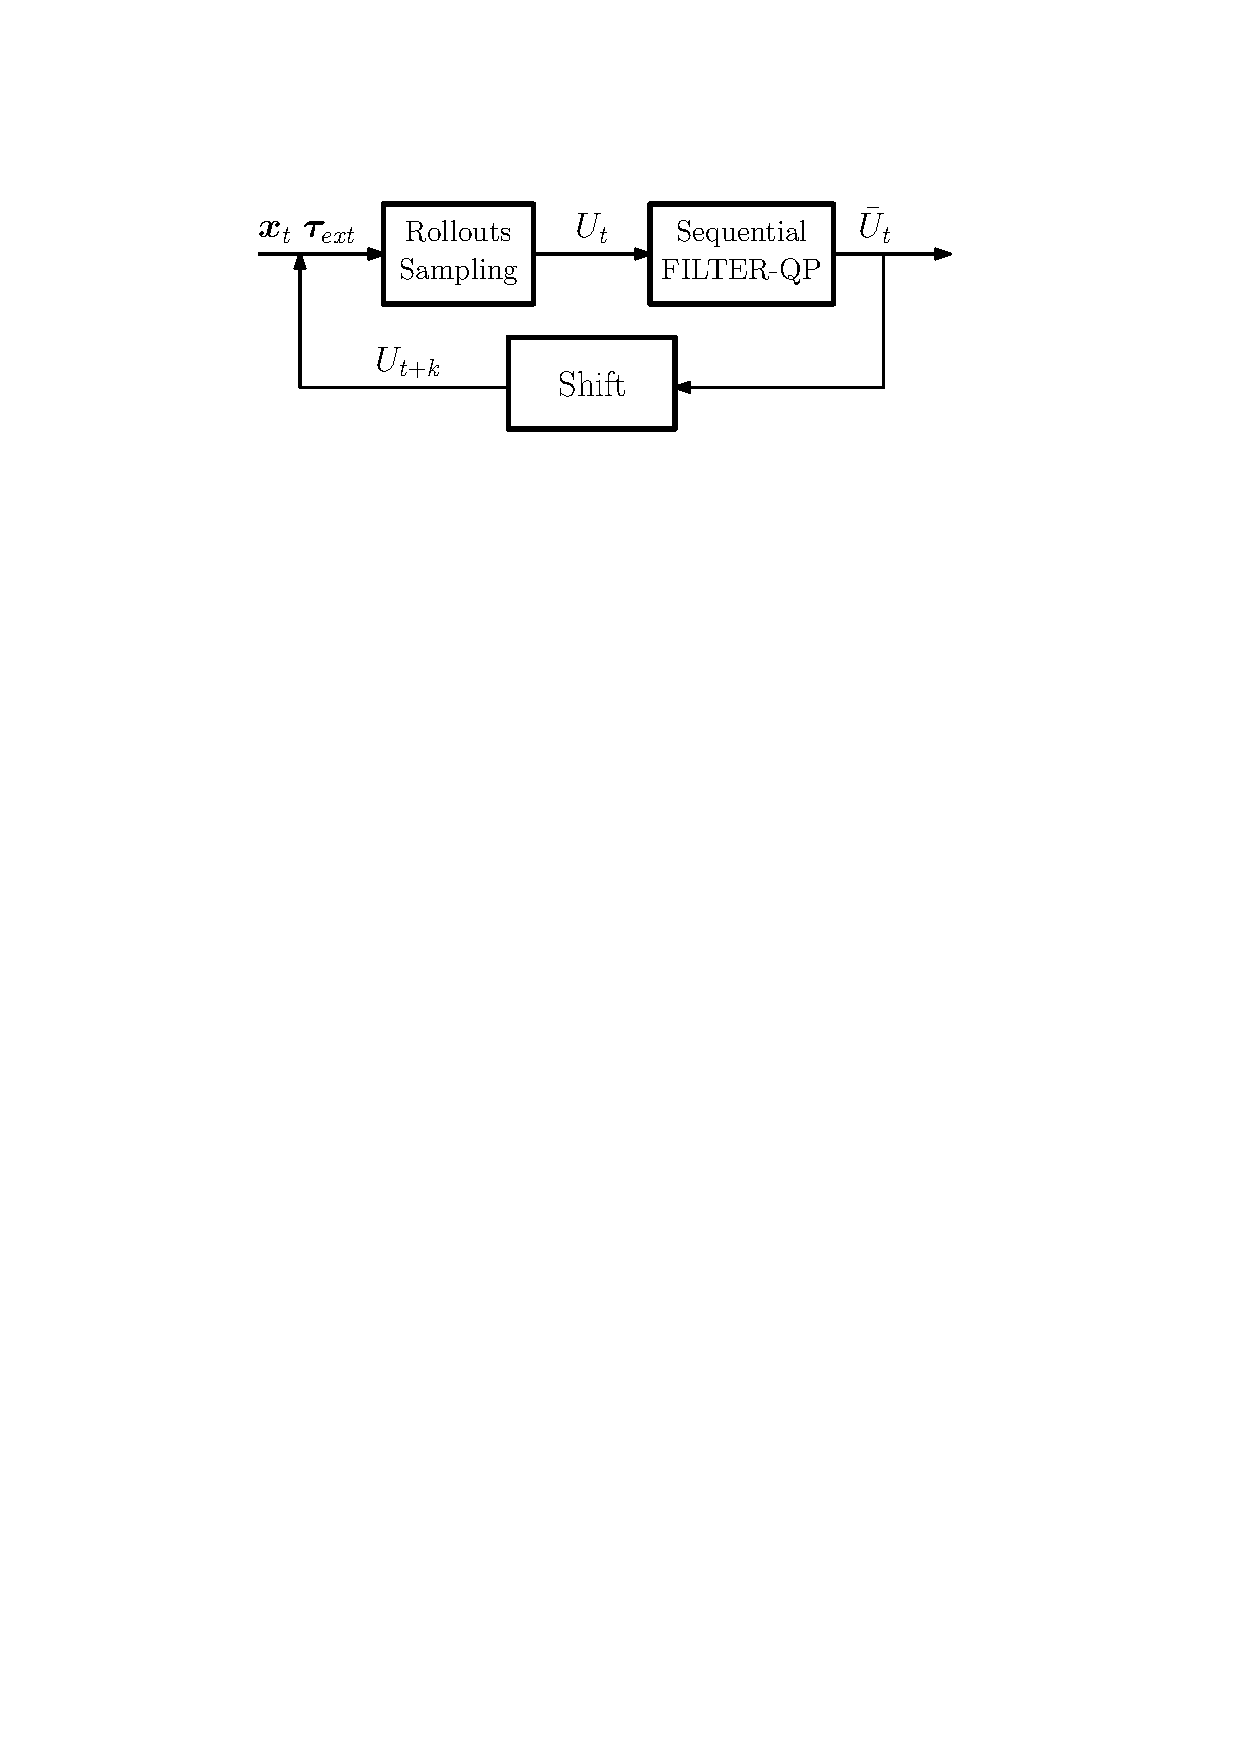
\includegraphics[width=0.8\columnwidth]{figures/schemes/stochastic_controller.pdf}
\caption{The sampling scheme is refined using the Sequential QP. The newly filtered trajectory is shifted in time and used to warm start the next sampling round.} \label{fig:sampling_scheme}
\end{figure}


\section{Practical Aspects} \label{sec:practical_aspects}

We address here some issues that arise when implementing the described algorithm on a resource-constrained platform. Furthermore, we introduce many practical expedients that deal with limited sampling budget, slow control rates and finally with sim-to-real transfer.  

\subsection{Gradient Clipping} 
The policy update rule in \eqref{eq:update_rule} consists of a receding horizon \emph{mini-batch} SGD. As a consequence, the gradient variance can vary greatly between successive iterations of the algorithm. To prevent this phenomenon, which is especially evident with a small sampling budget, we clip the gradients to a user-defined threshold.  

\subsection{Likelihood mapping} 
The coefficient $\lambda$ in \eqref{eq:weighting} determines how much ``aggressive" the weighting between different trajectories is. Adopting a constant value would give a numerically zero weight to most of the trajectories. Shifting the trajectory cost by the minimum cost as proposed in~\cite{williams_information_2017} also does not alleviate this issue. 
Especially in regions of high cost, trajectories that are equivalently good can be assigned very different weights. We instead propose to adopt the same technique as in~\cite{theodorou2010generalized} where the $\lambda$ is scaled to better discriminate between the experienced trajectories. The modified exponential utility is then defined by,
\begin{equation} \label{eq:scale_invariant_mapping}
    \exp (-\lambda J ) = \exp \left( -h \frac{J - J_{\min}}{J_{\max} - J_{\min}} \right).
\end{equation}
which has the nice property of being invariant to the cost scale. Assume for example, that in a target reaching task, the goal pose is far away and thus the cost incurred by each sampled rollout is scaled by a common scalar factor. This factor would disappear when using the previous equation for mapping rollouts to likelihood. We show the effect of cost-scale invariance in \fig \ref{fig:exponential_mapping_comparison}. In the figure we assume that samples' costs are uniformly distributed in the range between minimum and maximum cost and that the minimum cost shows a $20$\% reduction with respect to the worse rollout\footnote{This is a reasonable choice since we are in a online setup and we assume to be in a low sampling budget regime.}. We compare the exponential mapping $\mathcal{J} = \exp(-\lambda J)$ (\textit{naive}), with baseline reduction $\mathcal{J} = \exp(-\lambda (J - J_{min}))$ (\textit{baseline}) and the mapping in \eqref{eq:scale_invariant_mapping} (\textit{invariant}).

\begin{figure}[t]
    \centering
    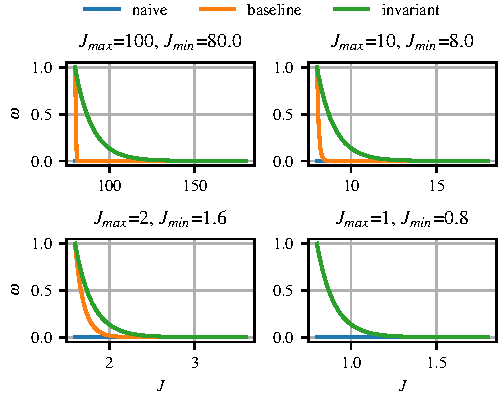
\includegraphics{figures/likelihood_mapping.pdf}
    \caption{In each plot we change the maximum and minimum cost ($80$\% of maximum cost). We set $\lambda$ and $h$ to 10 in all comparison.}
    \label{fig:exponential_mapping_comparison}
\end{figure}

When the cost is high, the first two methods collapse all the weight to a single sample and in practice, other samples are assigned a value which is numerically zero. As a consequence, the gradient estimate in \eqref{eq:update_rule} can show a high variance. The mapping in \eqref{eq:invariant_mapping} instead, assigns a non-zero weight to more samples independently from the current cost scale and helps to stabilize the gradient estimate.

\subsection{Chattering}
We observed that a naive implementation of the passivity constraint leads to a chattering behavior at the constraint boundary. We start discretizing the constraint inequality to obtain a constraint which is affine in the input $\command$:
\begin{equation*}
    \int_{0}^{t + dt} \boldsymbol{\tau}_{ext}^T \command \ dt \approx \underbrace{\boldsymbol{\tau}_{ext}(t)^T \command(t) dt}_{-P_{diss}} + S(x_t(t)) \geq \epsilon,
\end{equation*}
which is equivalent to 
\begin{equation} \label{eq:passivity_simple}
    P_{diss} \leq \alpha E_{res},
\end{equation}
where we defined the residual energy $S(x_t(t))-\epsilon$ as $E_{res}$. The above inequality has the drawback that when the Euler integration is performed with small time intervals, then a dangerously high power can be dissipated at any time, until very close to the lower energy limit, thus leading to chattering. It is therefore better to use a value of $\alpha < 1/dt$. Furthermore, one can easily verify that defining a passivity ZBF as $h_{pass} = S(x_t) - \epsilon$ we obtain the same formulation. The ZBF constraint reads as:
\begin{equation*}
    \dot{h}_{pass} = \dot{S}(x_t) \geq -\alpha h_{pass}
     =\alpha (\epsilon - S(x_t))).
\end{equation*}
The passivity can therefore seen as a ZBF and consequently inherits its properties. A smaller value for $\alpha$ makes the constraint more conservative and improves its performance at the boundary. In the worst case scenario, the dissipated power is always equal to the maximal power allowed by the passivity constraint: $\dot{E}_{res} = - \alpha E_{res}$. Then $E_{res}(t) = E_{res}(0) e^{-\alpha t}$. A smaller $\alpha$ makes the energy drop more slowly and avoids a fast depletion of the tank as shown in \fig \ref{fig:worst_case_energy_profile}.
\begin{figure}[t]
    \centering
    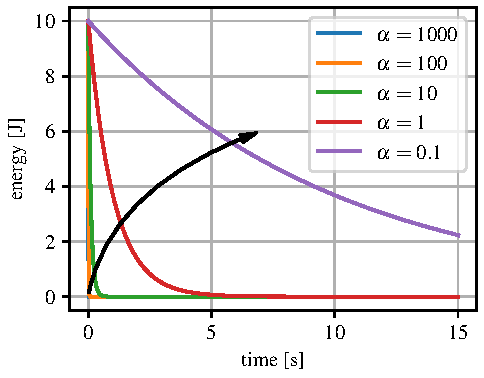
\includegraphics[width=0.8\columnwidth]{figures/worst_case_energy_profile.pdf}
    \caption{The figure shows the \textit{worst case} tank energy profile which is how the energy in the tank would evolve if the maximum allowed energy would be dissipated. The smaller the $\alpha$ and the more conservative is the constraint and the energy is depleted at a lower rate.}
    \label{fig:worst_case_energy_profile}
\end{figure}

This effect is shown in \fig \ref{fig:tank_as_zbf} in the experiment section.

\subsection{Sampling strategy}
At each control step, it is desirable to sample a zero input trajectory, meaning that all velocity commands are $\command_t = \bm{0} \forall t$ as this would allow the robot to stop when the goal is achieved. Similarly, we would like to keep sampling the unperturbed nominal command trajectory. In fact, if we assume this to be optimal for a time instant, re-sampling would perturb it and likely increase its associated cost. With this motivations in mind, we modify the sampling procedure such that there is always an unperturbed and zero velocity profile in the samples batch.

\subsection{Simulator tuning}
Crucial to the overall performance is the accuracy of the simulation environment (implementing \eqref{eq:eom}). Unfortunately the discrepancy between the simulator and the real physical model known as the \emph{sim-to-real} gap is always present. A typical failure case consists of an over-estimation of an object's friction. In such cases, we have often observed a ``scratching" emergent behavior where the robot would rely on friction to move the object. In practice friction is hard to measure and depends on the contact patch between surfaces. On the other hand, kinematic constraints between contact points depends on the system geometry which can be accurately measured (e.g from CAD models). Therefore solutions that exploit the latter are more likely to succeed on the real platform. One can bias the controller towards these solutions by setting, for example, a very low friction coefficient between contact bodies.

\subsection{Contact-mesh simplification}
A large proportion of simulation time is spent on collision detection. We reduce the component meshes to the relevant ones and simplify to primitive shapes, as shown in \fig\ref{fig:1}. We are especially interested in the collision objects belonging to the robot end-effector and the object. This adaptation tremendously reduces computation especially during the contact phase. In our following evaluations we observed that using the original mesh shown in \fig\ref{fig:original_mesh} results in a mean simulation rate of 0.98kHz. In contrast, the two finger mesh and hook finger mesh in \fig\ref{fig:two_fingers}-\ref{fig:hook_finger} allow mean simulation rates of 2.13kHz and 2.94kHz, respectively.

\begin{figure}[t]
\centering
\begin{subfigure}{0.3\columnwidth}
    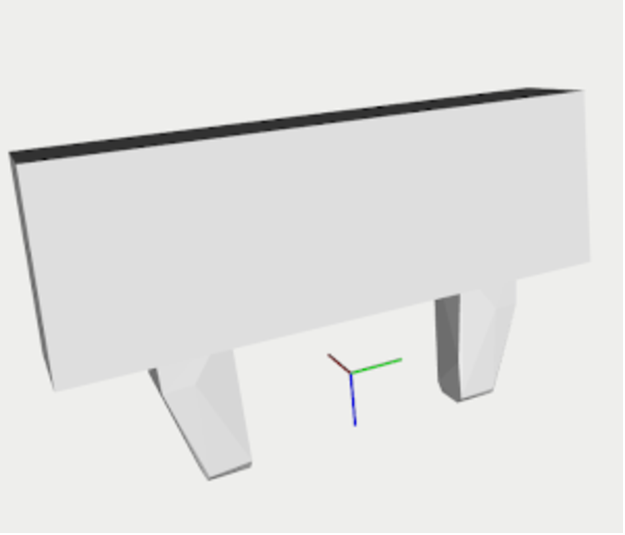
\includegraphics[width=\linewidth]{framework_manipulation/figures/hardware/mesh_cropped.pdf}
    \caption{Original mesh}\label{fig:original_mesh}
\end{subfigure}%
\hfill
\begin{subfigure}{0.3\columnwidth}
    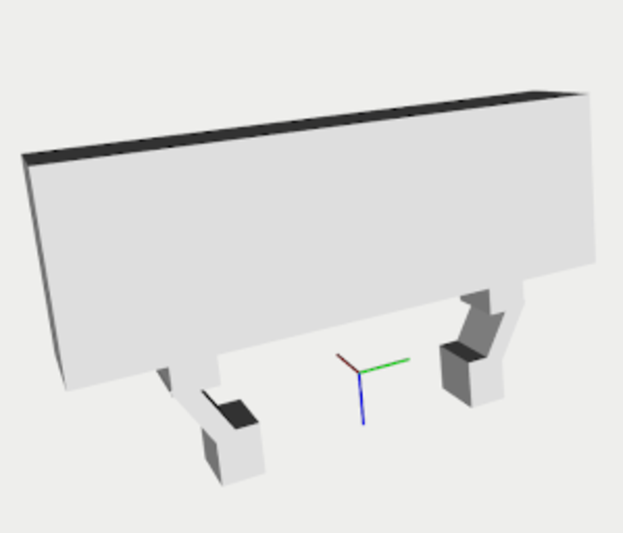
\includegraphics[width=\linewidth]{framework_manipulation/figures/hardware/doulbe_simple_cropped.pdf}
    \caption{Two fingers}\label{fig:two_fingers}
\end{subfigure}%
\hfill
\begin{subfigure}{0.3\columnwidth}
    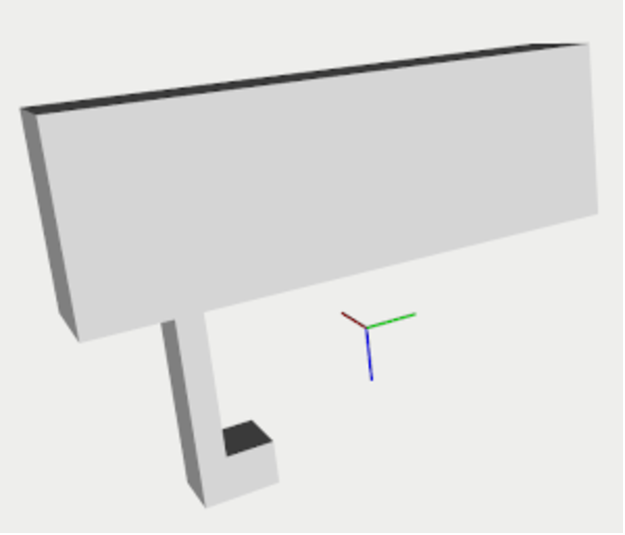
\includegraphics[width=\linewidth]{framework_manipulation/figures/hardware/single_hook_cropped.pdf}
    \caption{Hook finger}\label{fig:hook_finger}
\end{subfigure}

\caption{Original collision meshes are often approximated by convex hulls which are inaccurate while also more complex representations. In contrast, a simplified mesh can bring more accuracy as well as a computational performance gain in terms of simulation rate.}\label{fig:1}

\end{figure}



\section{Experimental Results} \label{sec:experiments}

The goal of this section is to investigate the limits of the naive sampling method which serves as benchmark for the proposed control framework. To this end, we define the following metrics:
\begin{itemize}
    \item \textit{average stage cost}: this performance metric is computed averaging the stage cost evaluated at each time step. Task duration and cost scheduling is kept fixed among all the experiments.  
    \item \textit{cumulative constraints violation}: as each barrier function is, by definition, negative outside of the safe set, we define the following metric as a proxy to the size of the constraint violation along the duration of an experiment:
    \begin{equation*}
        v^{tot}_i = \sum\limits_{t=0}^{T_{exp}} \max(0, -h_i(\vect{x}_t))
    \end{equation*}
    referring to the i\textsuperscript{th} barrier function and associated constraint.
    \item \textit{average interaction wrench}: average wrench which is exerted to the environment during the execution of the task
    \item \textit{dissipated power}: during an ideal interaction with an articulated object, power is not dissipated, meaning that the control doesn't act against the environmental constraint. We use the dissipated power as an efficiency metric:
    \begin{equation}
        P_{diss} = \sum\limits_{0}^{T_{exp}} -\command^T \boldsymbol{\tau}_{ext}
    \end{equation}
\end{itemize}
The simulation experiments are conducted on a dynamic manipulator model as described by \eqref{eq:eom}. The manipulation tasks consist in maneuvering different articulated objects. The articulated objects in the task are a \textit{shelf}, \textit{dishwasher}, \textit{microwave} and \textit{drawer} as shown in \fig\ref{fig:object_manipulation}. They differ in type and orientation of the joint. The \textit{shelf} and \textit{microwave} have a vertical revolute joint while the \textit{dishwasher} has a horizontal revolute joint. Ultimately, the \textit{drawer} has a horizontal prismatic joint. As the goal is to reproduce as close as possible the real manipulator, the simulation is run with a rate of 1000 Hz. The simulated manipulator is controlled using a PI velocity low-level controller, as its real counterpart and we model imperfect velocity tracking assuming that non-linear terms are not perfectly compensated. 
  
\begin{figure}[t]
\centering
  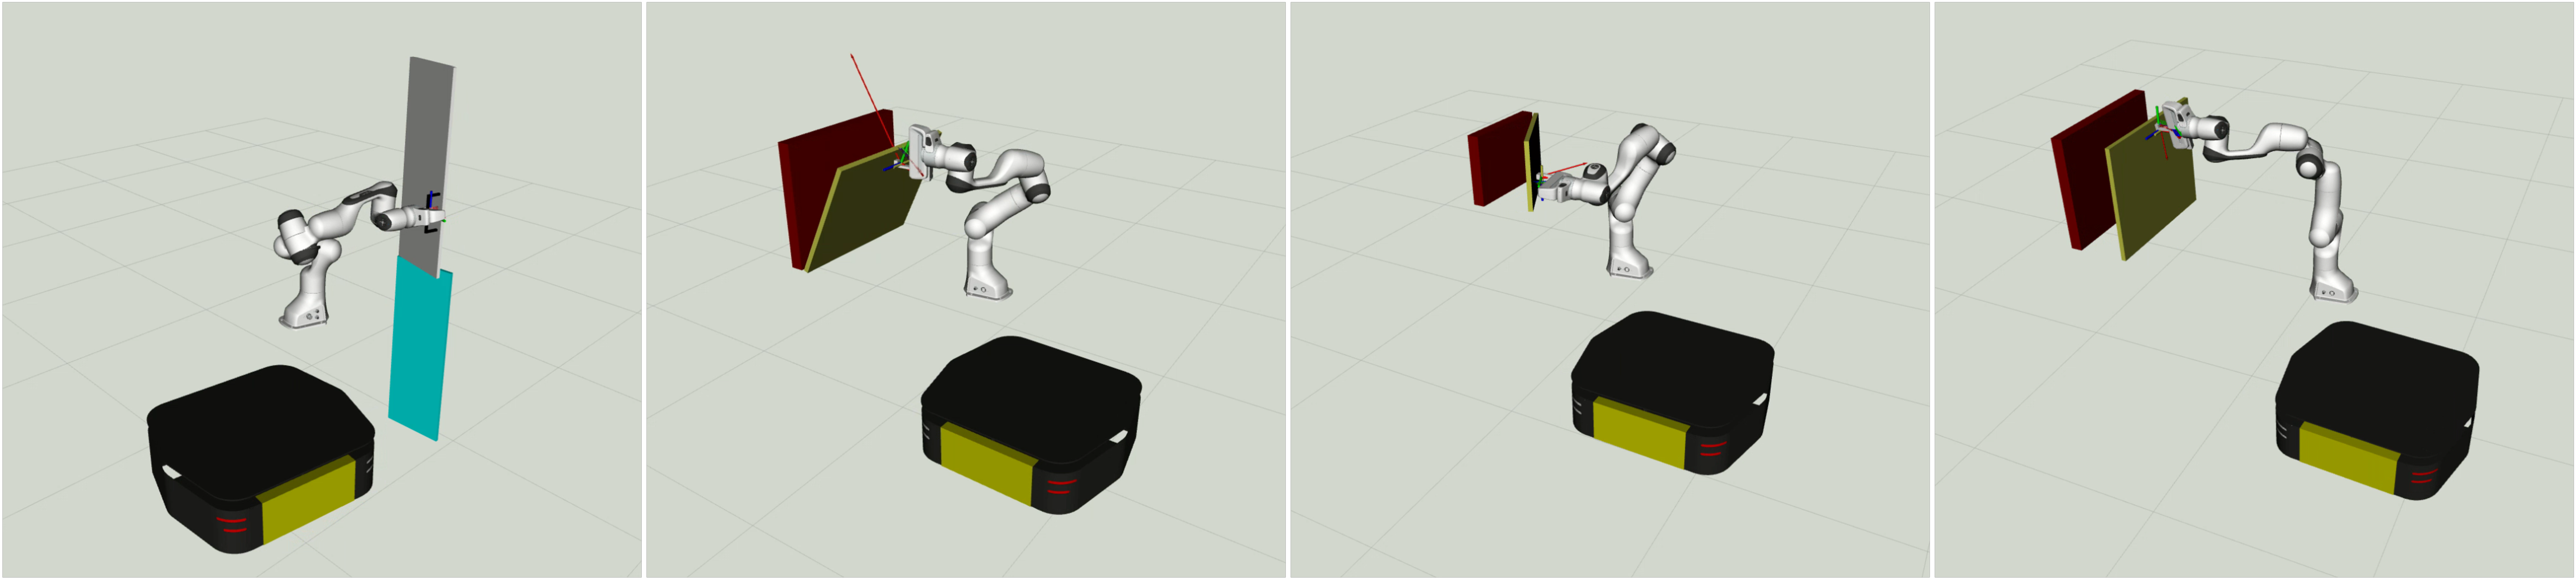
\includegraphics[width=\columnwidth]{figures/articulated_objects_sim.pdf}
  \caption{The four articulated objects used in our simulation evaluations. From left to right: shelf, dishwasher, microwave, drawer.} \label{fig:object_manipulation}
\end{figure}

\subsection{Power consumption}
In this experiment we look at the effect of the power term in the task execution. As we can see in \fig \ref{fig:power_cost_comparison}, the power cost is effective in decreasing the energy dissipation during the manipulation task. For each of the experiments where the power cost is active we set $w_p=10$ and $p_{max} = 0.0$. For all experiments we use $50$ samples as they are a good trade-off between control-frequency and performance. We observe that in all experiments the robot is able to accomplish the task (fully open the articulated object). This experiment shows that we can use wrench information to encode even more complex tasks. One for example, can think of shaping an \textit{information-theoretic} cost that seek useful wrench measurement to estimate the system model (TODO repharse or put in future works). 

\begin{figure}[t]
\centering
  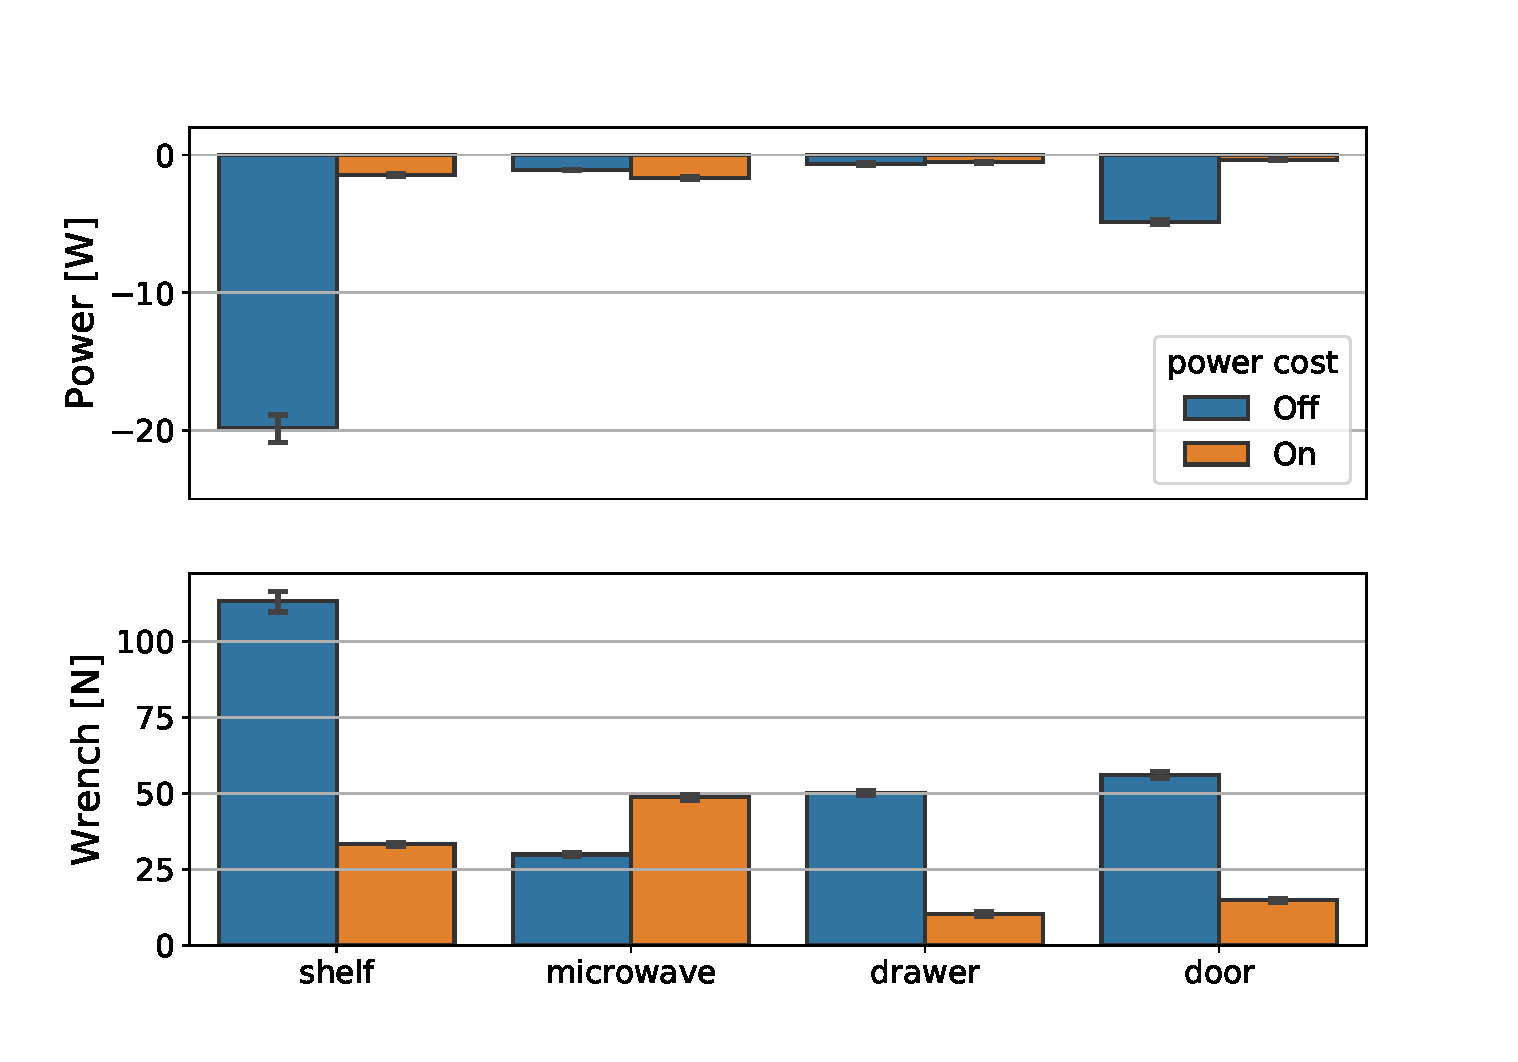
\includegraphics[width=\columnwidth]{figures/methods_comparison/power_cost.pdf}
  \caption{The first figures shows the power dissipated and wrench norm distribution for each manipulated object. As a beneficial side effect also the interaction wrench is reduced. Only for the microwave this is not the case but we see that even without this cost term, sampling is enough to find \textit{low power} trajectories.} \label{fig:power_cost_comparison}
\end{figure}


\subsection{Methods comparison}
We aim to compare the control framework in a challenging interaction scenario. In all the experiments the robot starts in configuration which is close to the arm joint limits and self collision. The base of the robot is at $(-3.0, -3.0)$ outside of the prescribed position limits of $[(2.0, 2.0), (-2.0, -2.0)]$. We perform ten experiments for each articulated object and we compare four control methods:
\begin{itemize}
    \item \textit{no\textunderscore filter}: only sampling is used to generate velocity commands,
    \item \textit{filter\textunderscore out}: the velocity command is passed at every time step of the low-level controller through the FILTER-QP,
    \item \textit{filter\textunderscore in}: the velocity trajectory is passed through the FILTER-QP before being sent to the low-level controller. This is then fed back to the sampling procedure as described in \algo \ref{algo:sequential_qp},
    \item \textit{filter\textunderscore in\textunderscore out}: a combination of the previous two methods where the FILTER-QP is used to transform velocity trajectories and at a higher rate in the low-level control loop (see \fig \ref{fig:cascaded_architecture})
\end{itemize}
The results of the experiments are summarized in \fig \ref{fig:methods_comparison}. In all cases, filtering the velocity commands has a beneficial effect. The drastic reduction of cumulative joint limits violation shows that closing the loop between the filter and the sampling allows to react more quickly to constraints violation and suggests that we are able to generate trajectories that recover from constraints violation. We can observe also a reduction of the violation of self collision and reach constraints, but in this case the improvement of  \textit{filter\textunderscore in\textunderscore out} with respect to \textit{filter\textunderscore in} is not as prominent. We hypothesize that this is due to a low likelihood of getting into self-collision given the task and robot morphology. Considering dissipated power, we see that the overall trend is a more efficient task execution. Positive values for the shelf case, show that desired velocity has the same direction as the external force, resulting in a more compliant autonomous behavior. This will become more evident in the next experiment where we simulate a model mismatch which might lead to high interaction forces. 
\begin{figure}[t]
\centering
\hspace*{-0.4cm} 
\begin{subfigure}{\columnwidth}
    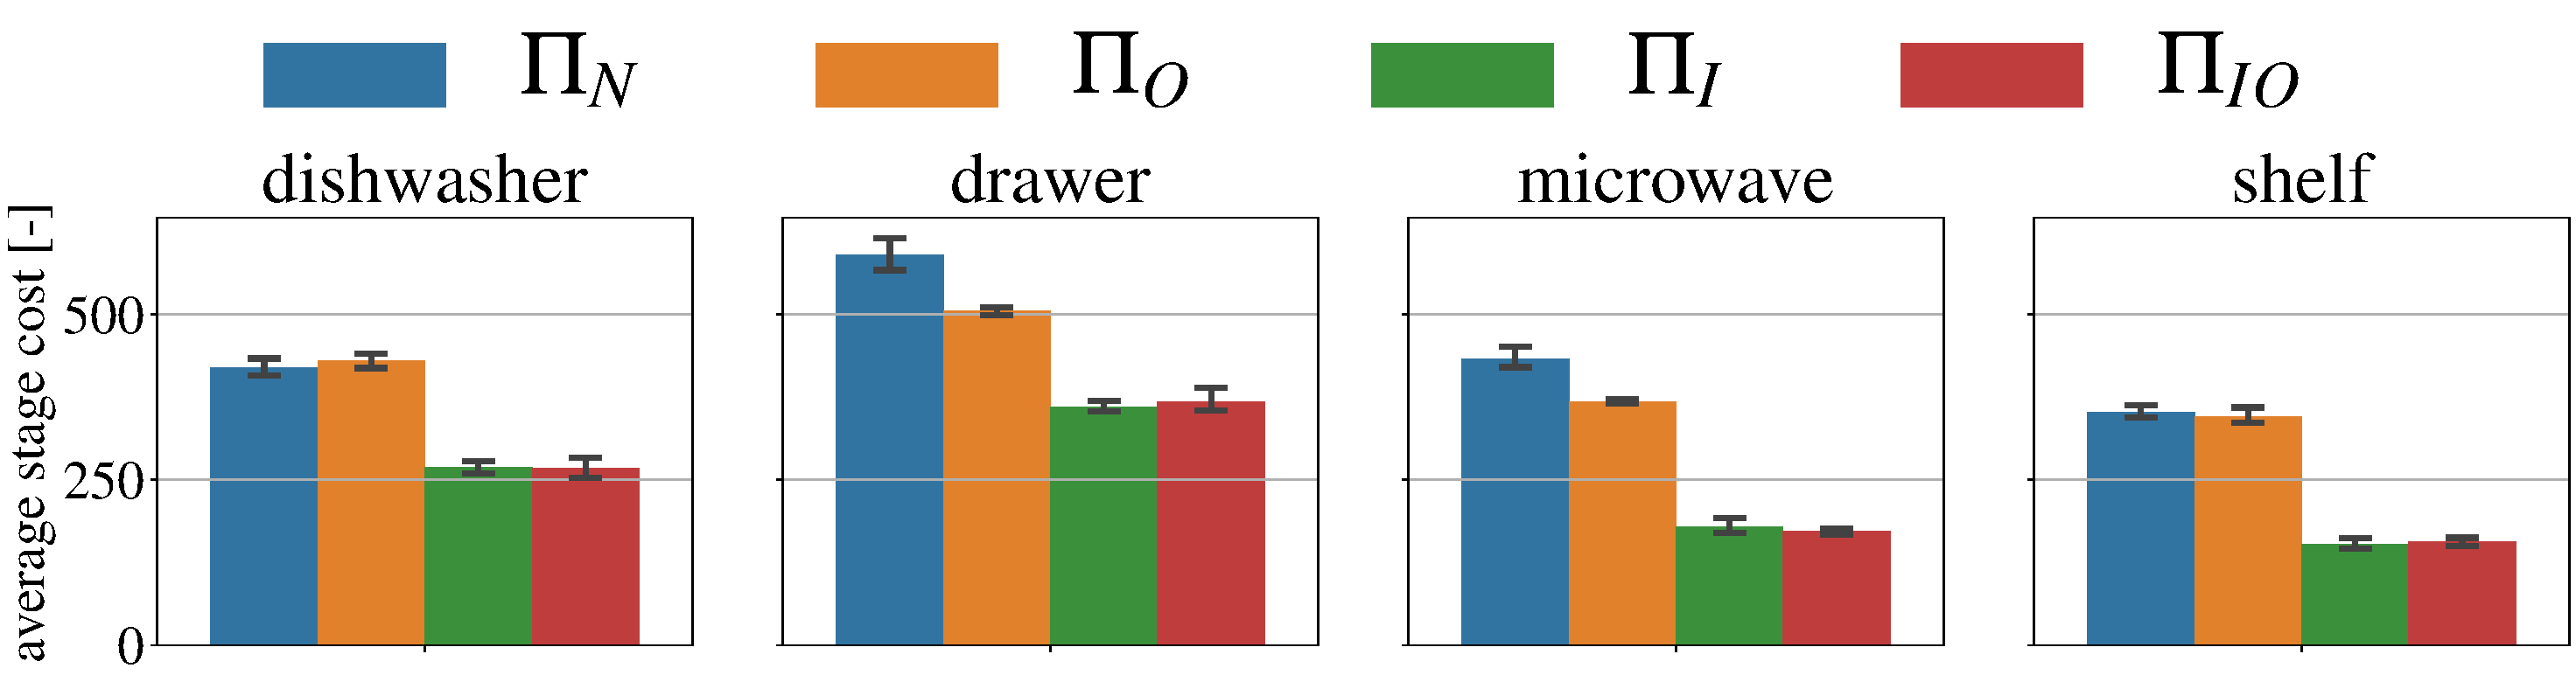
\includegraphics[width=\linewidth]{figures/methods_comparison/average_stage_cost.pdf}
\end{subfigure}%
\hfill
\hspace*{-0.4cm} 
\begin{subfigure}{\columnwidth}
    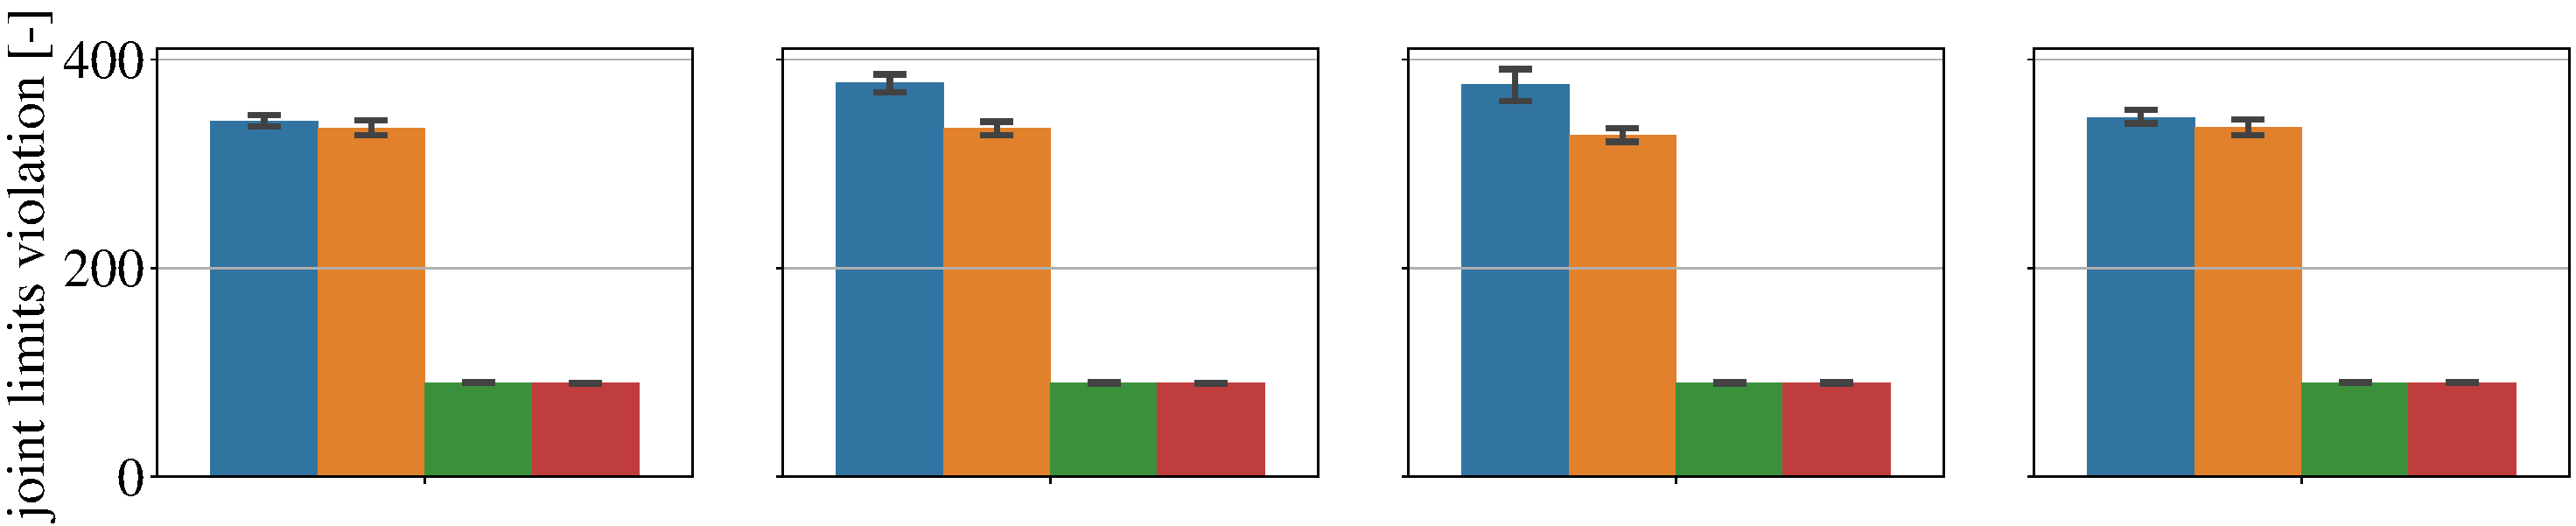
\includegraphics[width=\linewidth]{figures/methods_comparison/joint_limits.pdf}
\end{subfigure}%
\hfill
\hspace*{-0.4cm} 
\begin{subfigure}{\columnwidth}
    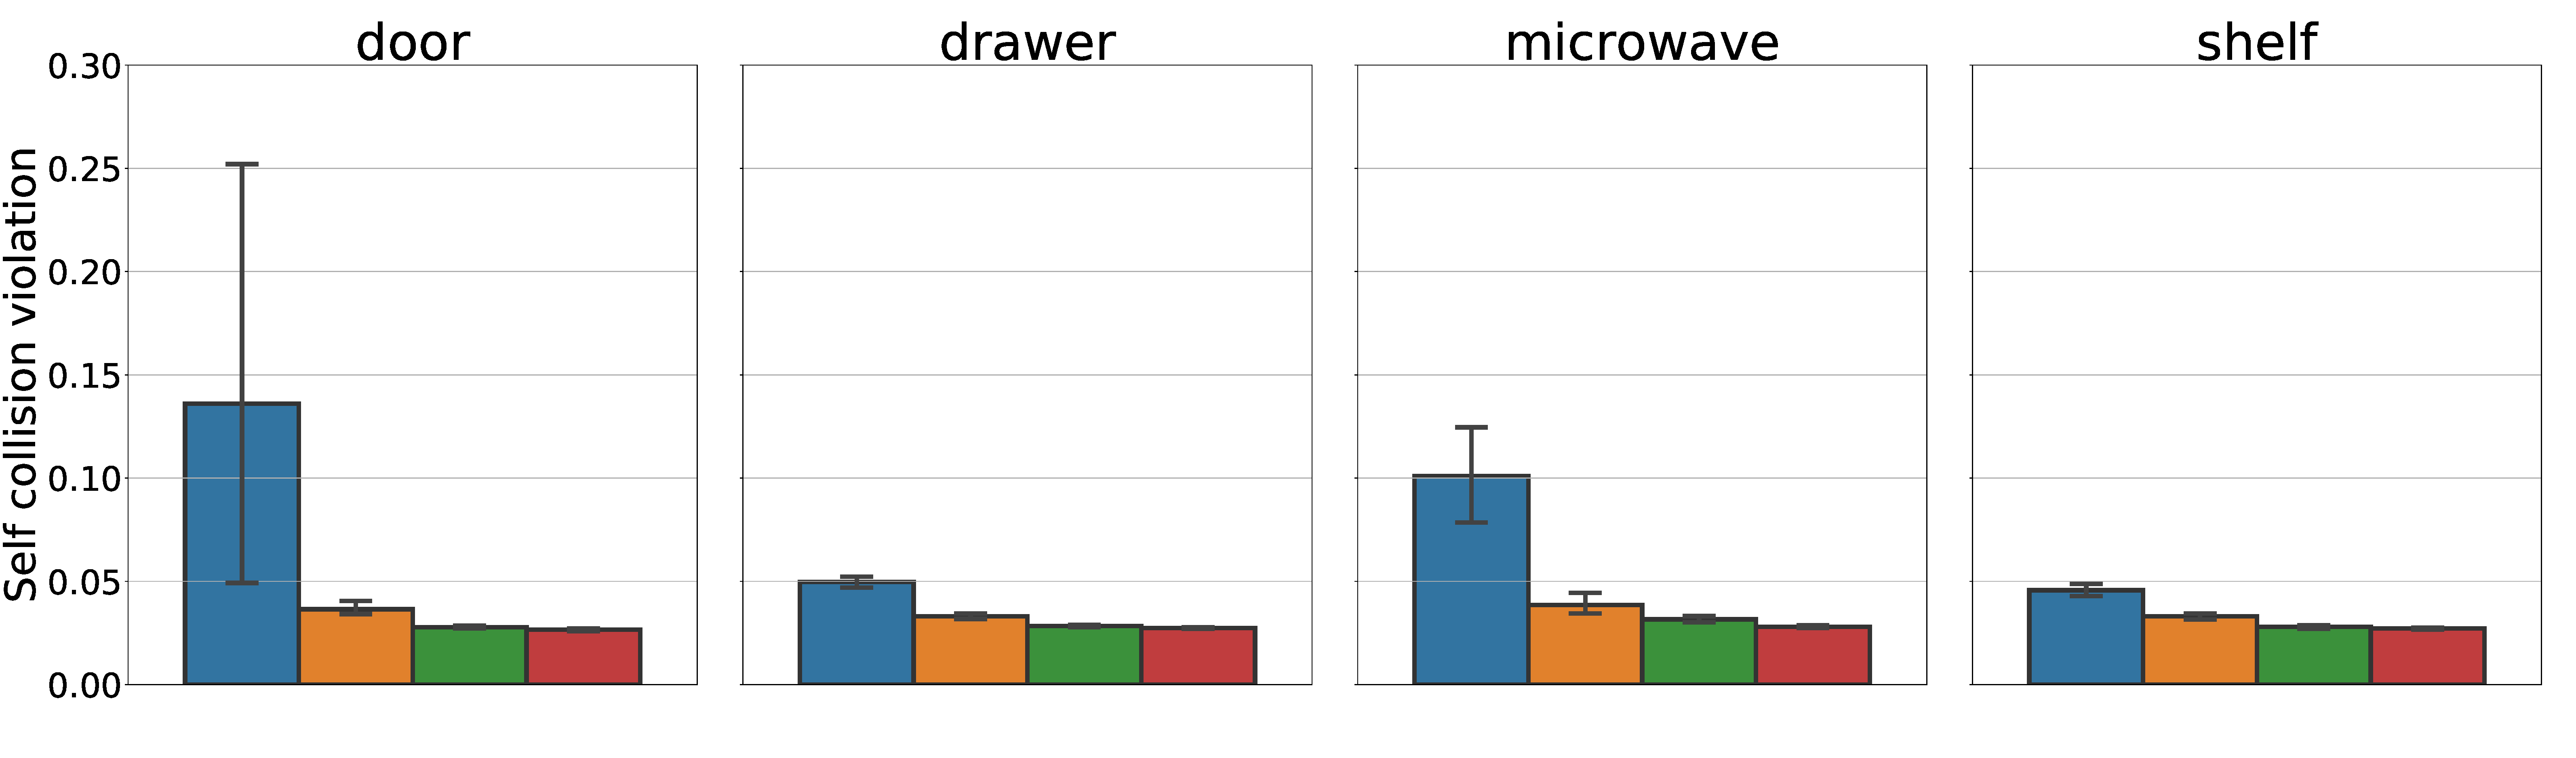
\includegraphics[width=\linewidth]{figures/methods_comparison/self_collision.pdf}
\end{subfigure}
\hspace*{-0.4cm} 
\begin{subfigure}{\columnwidth}
    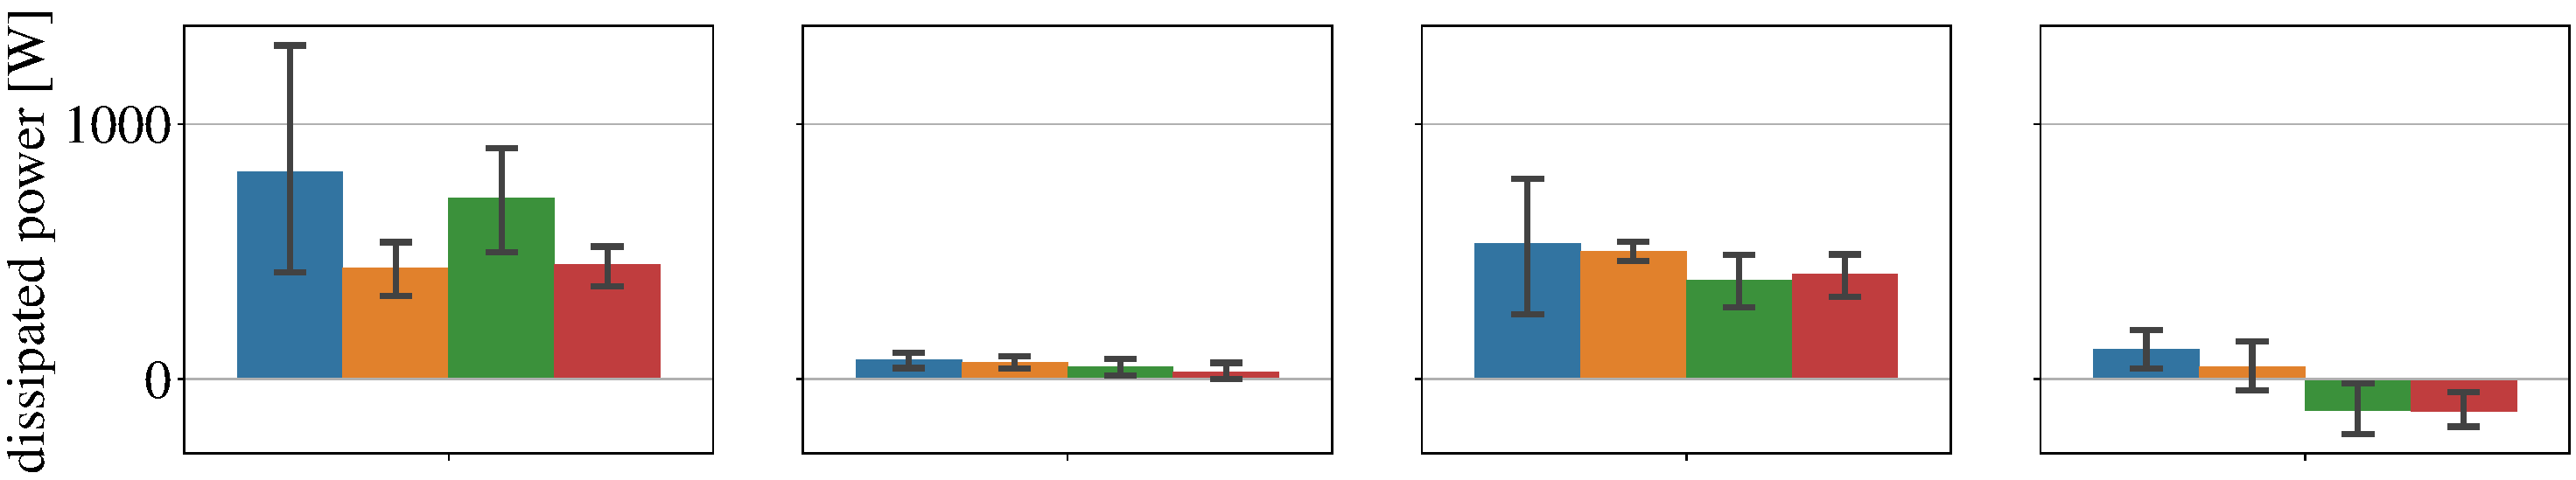
\includegraphics[width=\linewidth]{figures/methods_comparison/dissipated_power.pdf}
\end{subfigure}
\hfill
\caption{This figure shows a comparison between the different control methods when the FILTER-QP is used in different stages of the cascaded architecture. Results are separate by manipulation task. The self-collision metric accounts also for the arm-reach constraint as they share the same implementation.}\label{fig:methods_comparison}
\end{figure}

\subsection{Interaction wrench}
We want to investigate if the controller can reason about interaction wrench through the power cost described in \eqn \ref{eq:power_cost}. This is a novel algorithmic component, as it enables indirect control of the interaction wrench. 

\subsection{Robust interaction}
In this experiment we aim to show that the tank is effective in limiting the dissipated power and thus generating a stable and robust interaction behavior. We design an interaction scenario where the articulated object gets stuck during motion. In the simulated experiments we fix the object position for $5s$. After this time the object is release and free to move. We can note that when the SAFETY-QP is turned off and therefore no passivity is ensured, the negative power flow is not bounded, leading to high interaction wrenches. On the other hand, when the energy tank is used, only a maximal amount of energy, namely that stored in the tank can be used, regulating the overall interaction wrench.    

\begin{figure}[t]
\centering
\hspace*{-1.35cm} 
\begin{subfigure}{1.3\columnwidth}
    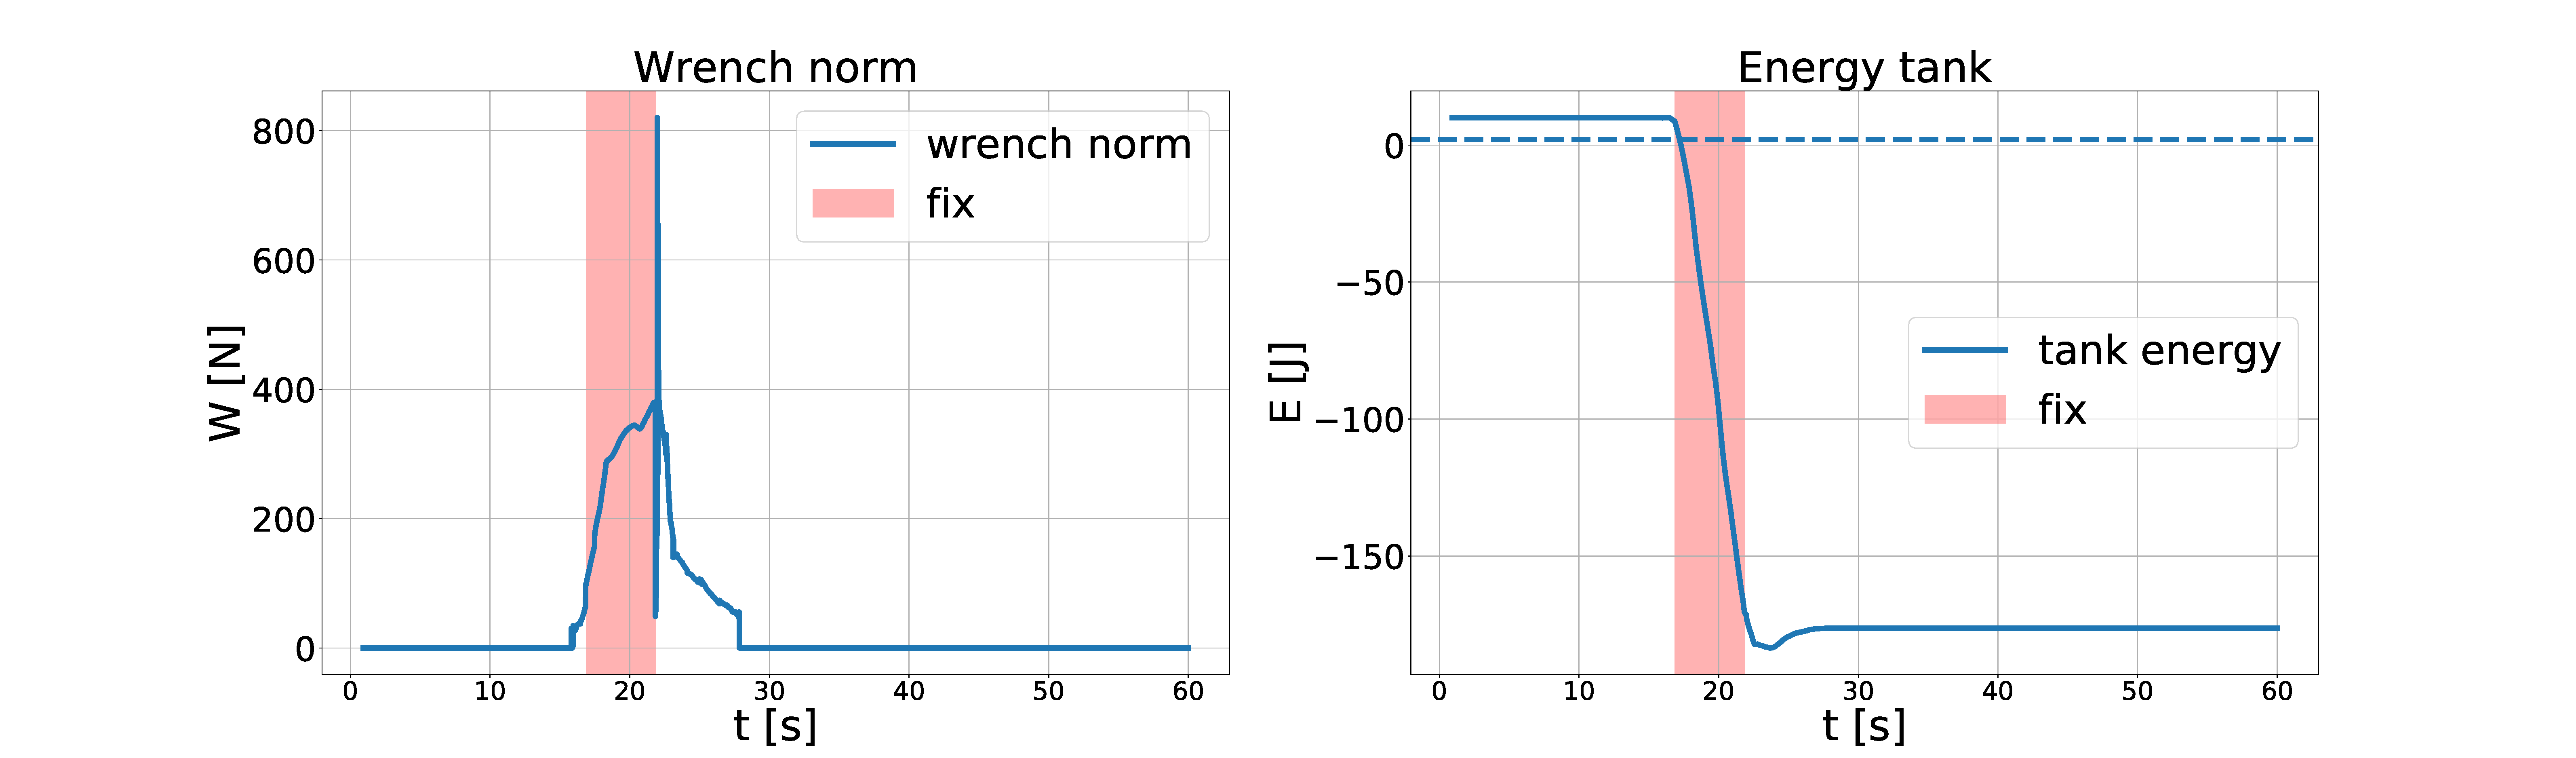
\includegraphics[width=\linewidth]{figures/fix_experiment/wrench_tank_without_tank.pdf}
    \caption{without tank}
\end{subfigure}
\hspace*{-1.35cm} 
\begin{subfigure}{1.3\columnwidth}
    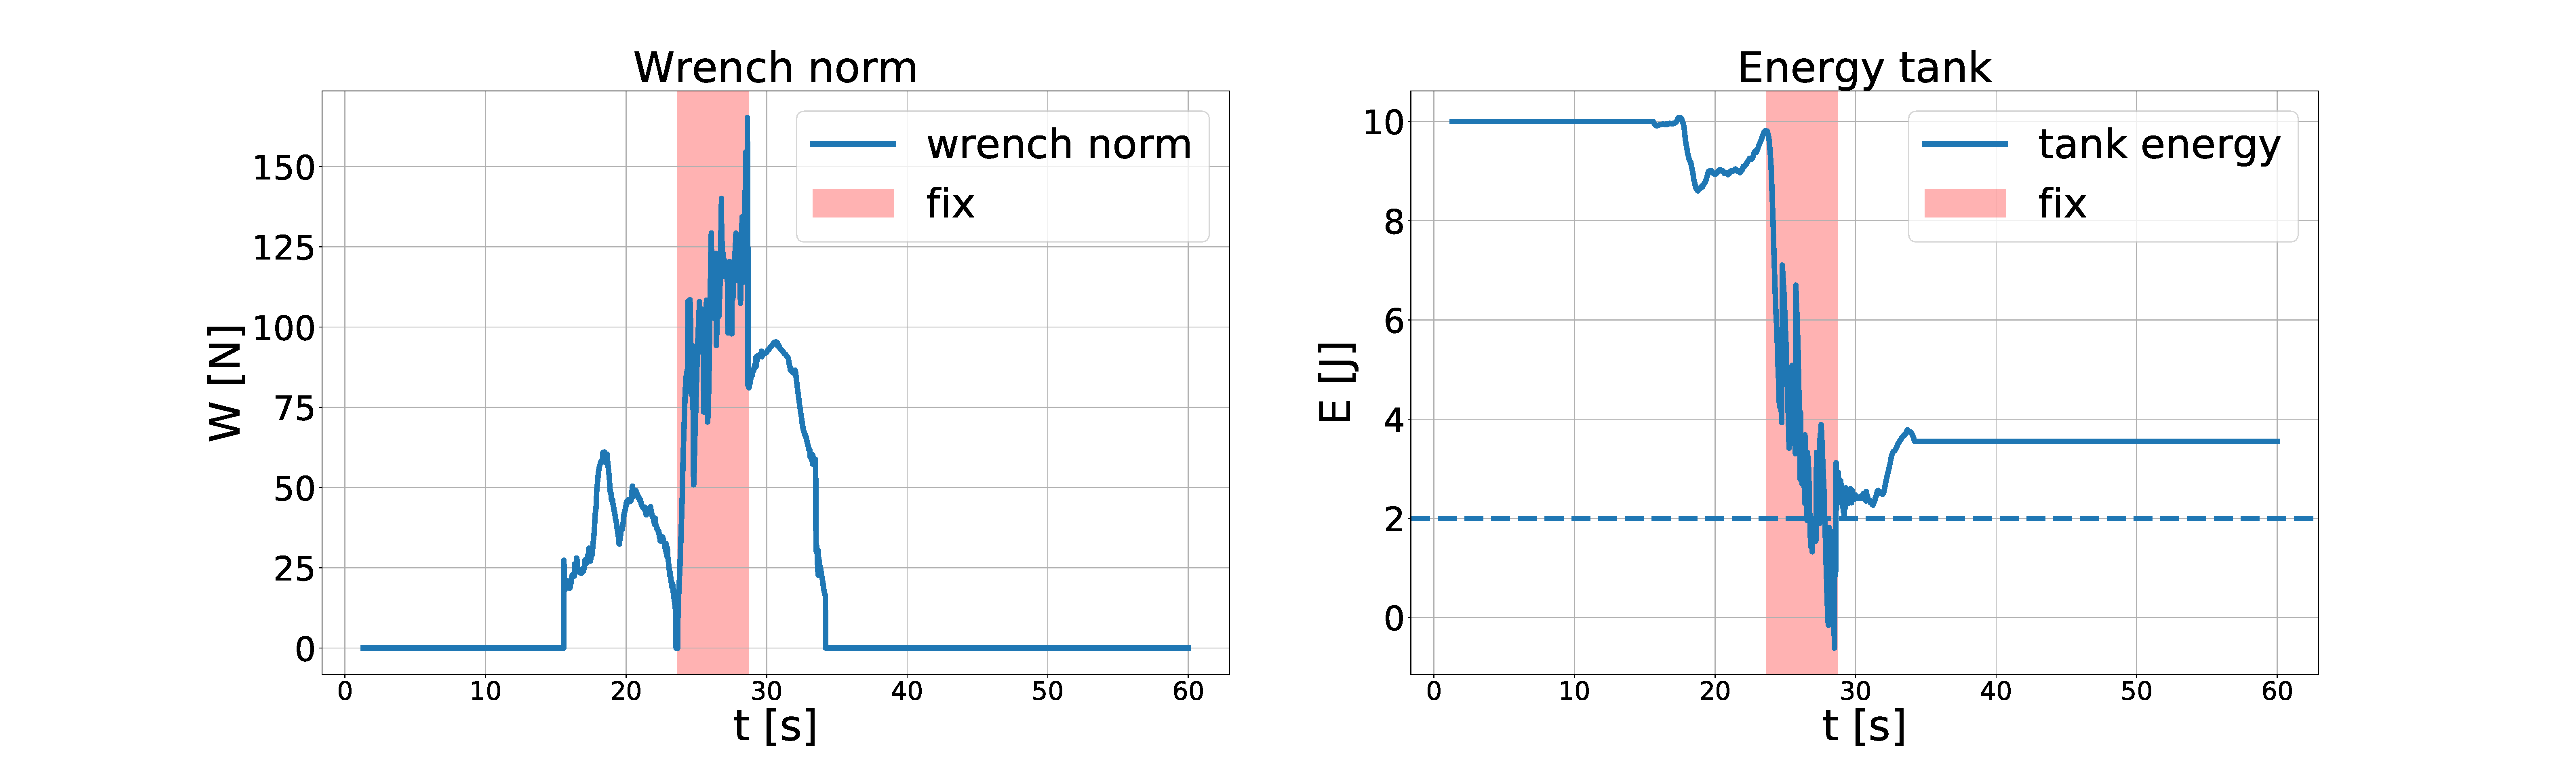
\includegraphics[width=\linewidth]{figures/fix_experiment/wrench_tank_with_tank.pdf}
    \caption{with tank}
\end{subfigure}
\hfill
\caption{The figure shows the interaction wrench and energy left in the tank during the task execution. The shaded area is the interval of time where the articulated object is fixed.  }\label{fig:methods_comparison}
\end{figure}
\subsection{Real world experiments}
Our RoyalPanda test platform consists of a holonomic mobile base equipped with a 7-DOF manipulator. The robot's wrist mounts a custom set of fingers as shown in \fig\ref{fig:custom_fingers}. This hardware adaptation simplifies the problem without limiting the capabilities of the platform. We run the presented algorithm on a Intel Core i7-8550U quad-core processor (1.8 GHz, up to 4.0 GHz) and use 8 threads for parallel forward sampling of rollouts. All control parameters are summarized in \tab \add{add table of parameters}. The target velocity commands are tracked by a PI controller which converts these into motor torques. The omnidirectional base is controlled by sending velocity commands to the mecanum wheel controller. The arm's low-level controller runs at 1KHz while the base mecanum controller runs at 50Hz.


The experiment goal is to demonstrate that the algorithm can be deployed on a real platform at high control rates. For this purpose, we perform a door opening experiment. The door and the robot base are tracked via a VICON system, eliminating the need for precise state estimation. We plan to remove this limitation in future work. In order to qualitatively evaluate the algorithm's replanning capabilities, we disturb the manipulator during the opening phase releasing the contact between the handle and the finger. As we can see in the accompanying video, the controller is able to re-plan a feasible trajectory to the handle and successfully perform the task.     
In \fig\ref{fig:mobile_manipulation_hardware} the magnitudes of the base and end-effector velocities are plotted to visualize the whole-body coordination throughout the manipulation task.

\begin{figure}[t]
\centering
\begin{subfigure}{\columnwidth}
    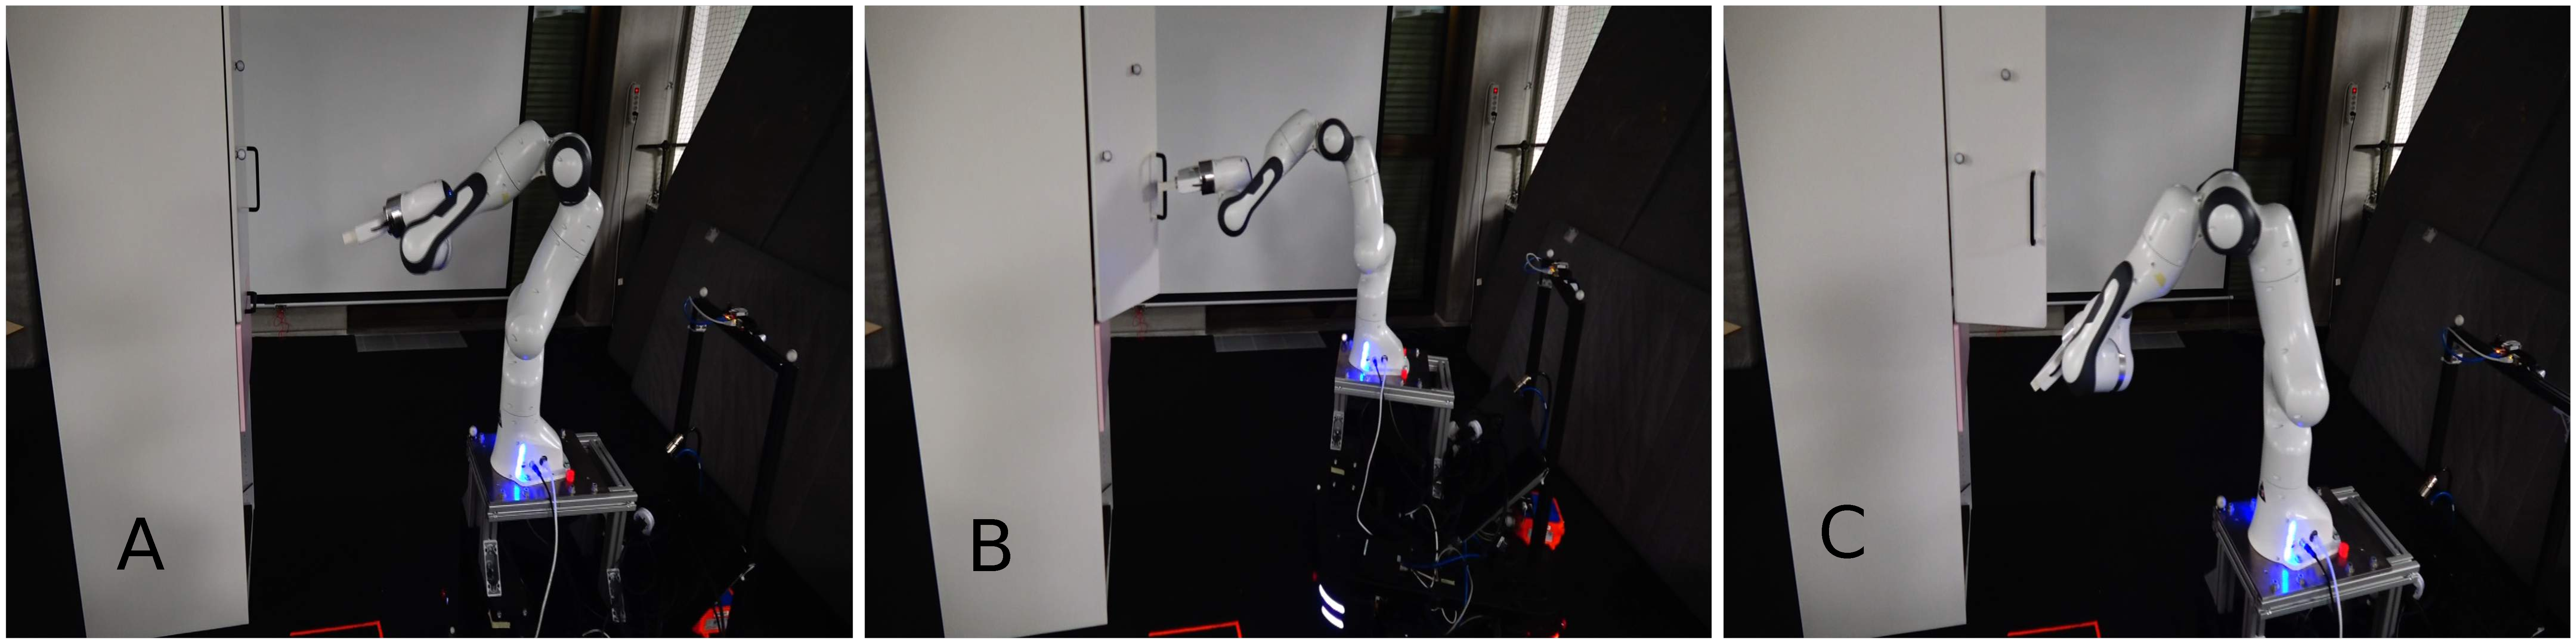
\includegraphics[width=\linewidth]{figures/mobile_robot_montage-compressed.pdf}
    \caption{Extract of the manipulation sequence. In A the robot reaches an estimated target region near the handle. In B the door is opened. In C the end-effector moves back to the starting pose.}
\end{subfigure}%
\hfill
\begin{subfigure}{\columnwidth}
    \includegraphics[trim={0 10 0 50},clip,width=\linewidth]{figures/velocity_norm_annotated.pdf}
    \caption{Velocity contributions of the base and of the end-effector with respect to the base frame. These results show that whole-body coordination occurs at all the times of the manipulation task.}
\end{subfigure}%}
\caption{Whole-body door opening with a mobile manipulator.} \label{fig:mobile_manipulation_hardware}
\end{figure}

\section{Conclusions} \label{sec:conclusions}

In this work, we have presented a novel control framework for interaction control. We have shown its applicability to the real platform and enhanced its robustness adding new algorithmic components which deploys ZBFs and passivity. We devised a cascaded control architecture which takes into account real-time constraints and applied for the first time these methods on a mobile manipulation platform in real-world experiments. The proposed solution is robust and guarantees stability and safety in case of unforeseen and sudden safety-critical events as we have demonstrated in our simulated and hardware experiments. Last but not least, we open source an efficient multi-threaded implementation of the algorithms that we hope can help practitioners to extend and use this method on new applications.


%Nevertheless there are still some interesting research directions that we aim to address in the near future. As any model-based control method, this is brittle to model mismatches. While stability is guaranteed through passivity, one could exploit interaction to find a better model estimate, closing the loop between perception and control. To this end, the haptic information readily available throughout the simulated rollouts could be actively used to drive an exploratory behavior. Another interesting idea is to use a policy parameterization other than a multivariate Gaussian such that sampling can be done more efficiently in a lower dimensional space. The proposed method is flexible enough to be applied to systems other than mobile manipulators. We hope that the released library will help in this process and with development of future applications. 


% \addtolength{\textheight}{-13.5cm}   % This command serves to balance the column lengths
                                  % on the last page of the document manually. It shortens
                                  % the textheight of the last page by a suitable amount.
                                  % This command does not take effect until the next page
                                  % so it should come on the page before the last. Make
                                  % sure that you do not shorten the textheight too much.

%%%%%%%%%%%%%%%%%%%%%%%%%%%%%%%%%%%%%%%%%%%%%%%%%%%%%%%%%%%%%%%%%%%%%%%%%%%%%%%%
% \section*{ACKNOWLEDGMENT}

% This work was supported in part by ABB Corporate Research, the Luxembourg National Research Fund (FNR) 12571953 and the ETH Foundation with an unrestricted gift from Huawei Technologies.


%%%%%%%%%%%%%%%%%%%%%%%%%%%%%%%%%%%%%%%%%%%%%%%%%%%%%%%%%%%%%%%%%%%%%%%%%%%%%%%%

\bibliographystyle{IEEEtran}
% argument is your BibTeX string definitions and bibliography database(s)
\bibliography{references}

%%%%%%%%%%%%%%%%%%%%%%%%%%%%%%%%%%%%%%%%%%%%%%%%%%%%%%%%%%%%%%%%%%%%%%%%%%%%%%%%
\section{Derivation of policy gradient}\label{sec:app_derivation_policy_gradient}
We aim to maximize the log-likelihood of the success variable $\success$. Recall that the optimization variables are the parameters of the current policy, namely the mean vector of the normally distributed control sequence $\policyParams$. 
\begin{align*}
    \nabla_{\policyParams} \log \succProb &= \nabla_{\policyParams} \log \expPolicy{\succCondProb} \\
    &= \frac{\nabla_{\policyParams} \expPolicy{\succCondProb}}{\expPolicy{\succCondProb}}.
\end{align*}
We further analyze the numerator of the previous expression and assume deterministic dynamics:
\begin{align*}
    \nabla_{\policyParams} \int \succCondProb \policy dU &= \int \succCondProb \nabla_{\policyParams} \policy dU \\
    &= \int \succCondProb \policy \nabla_{\policyParams} \log \policy dU \\
    &= \expPolicy{\succCondProb \nabla_{\policyParams} \log \policy},
\end{align*}
leading to the expected result. 


\section{Table of parameters}\label{app:table_of_parameters}

\begin{table}[h!]
\centering
\begin{tabular}{||c c c c||} \label{ta}
 \hline
 Col1 & Col2 & Col2 & Col3 \\ [0.5ex] 
 \hline\hline
 1 & 6 & 87837 & 787 \\ 
 \hline
 2 & 7 & 78 & 5415 \\
 \hline
 3 & 545 & 778 & 7507 \\
 \hline
 4 & 545 & 18744 & 7560 \\
 \hline
 5 & 88 & 788 & 6344 \\ [1ex] 
 \hline
\end{tabular}
\caption{Table to test captions and labels.}
\label{tab:parameters}
\end{table}


%%%%%%%%%%%%%%%%%%%%%%%%%%%%%%%%%%%%%%%%%%%%%%%%%%%%%%%%%%%%%%%%%%%%%%%%%%%%%%%%

% References are important to the reader; therefore, each citation must be complete and correct. If at all possible, references should be commonly available publications.








\end{document}
